\section{Comparing to Greedy Next-Best-View}
A course field of size $20 \times 20$ vesicles was generated with a autocorrelation factor, $\sigma_{field}$, equal to $4$, and limited to a $30\%$ scan.

\begin{figure}[htb!]
    \centering
    \begin{subfigure}[t]{0.3333\textwidth}
        \centering
        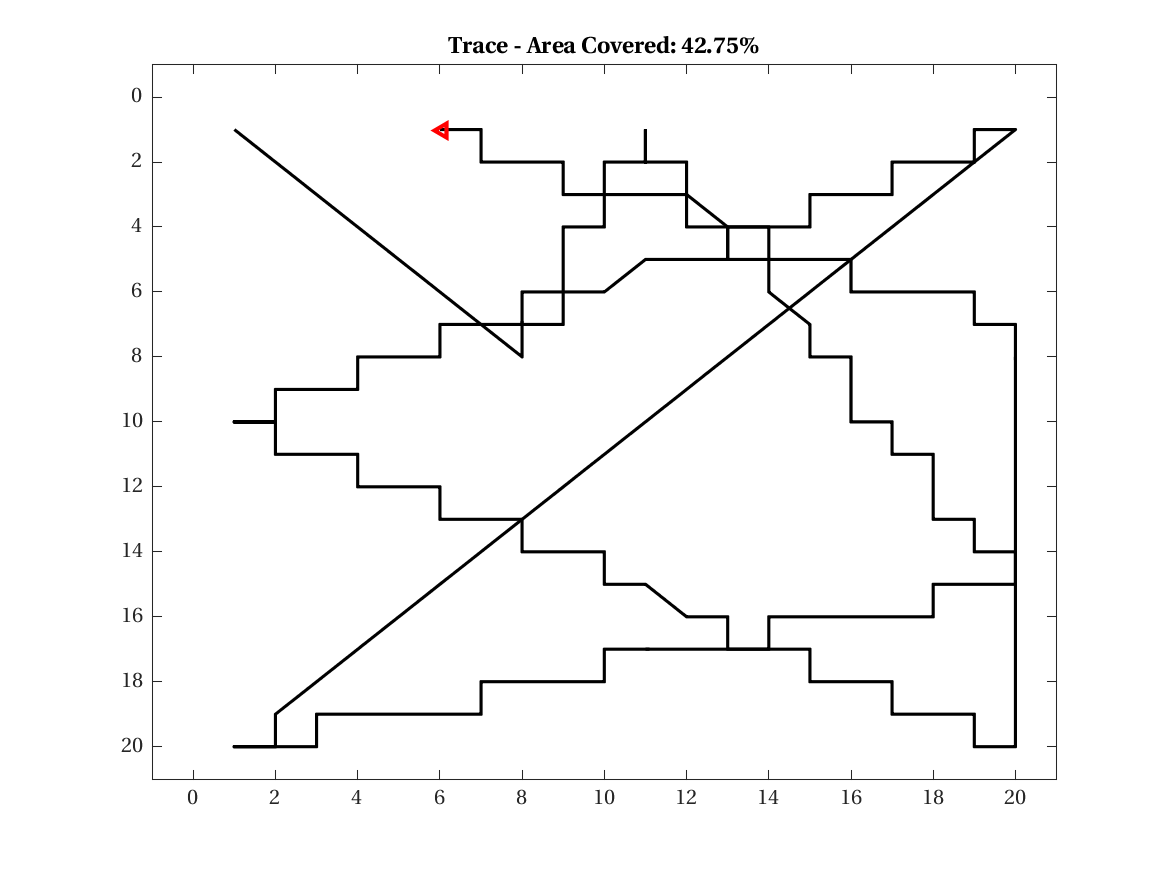
\includegraphics[width=\linewidth]{figures/hbresults/path_nhv_40p_20x20_sf_4_seed_2.png}
        \captionsetup{skip=0.20\baselineskip,size=footnotesize}
        \caption{Highest Variance}
    \end{subfigure}%
    \begin{subfigure}[t]{0.3333\textwidth}
        \centering
        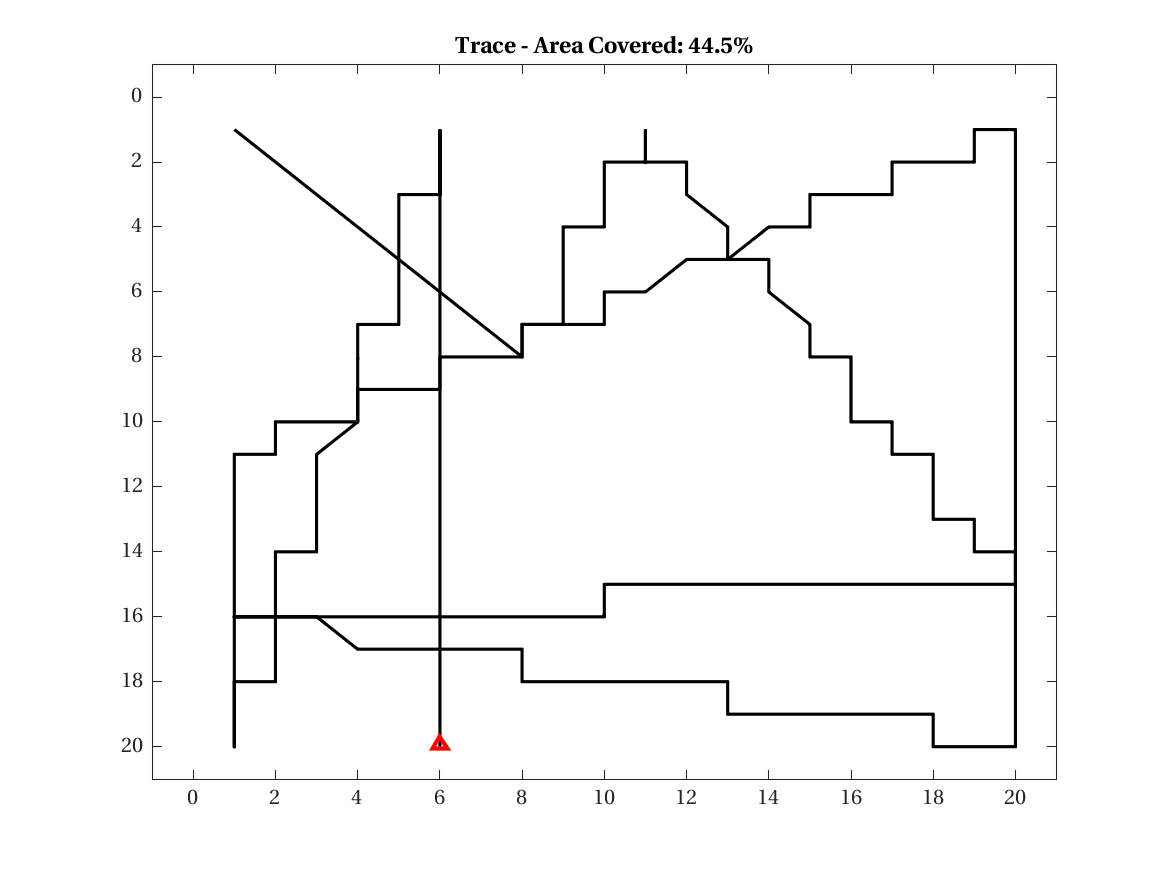
\includegraphics[width=\linewidth]{figures/hbresults/path_nnhv_40p_20x20_sf_4_seed_2.png}
        \captionsetup{skip=0.20\baselineskip,size=footnotesize}
        \caption{$N$ Highest Variance}
    \end{subfigure}%
    \begin{subfigure}[t]{0.3333\textwidth}
        \centering
        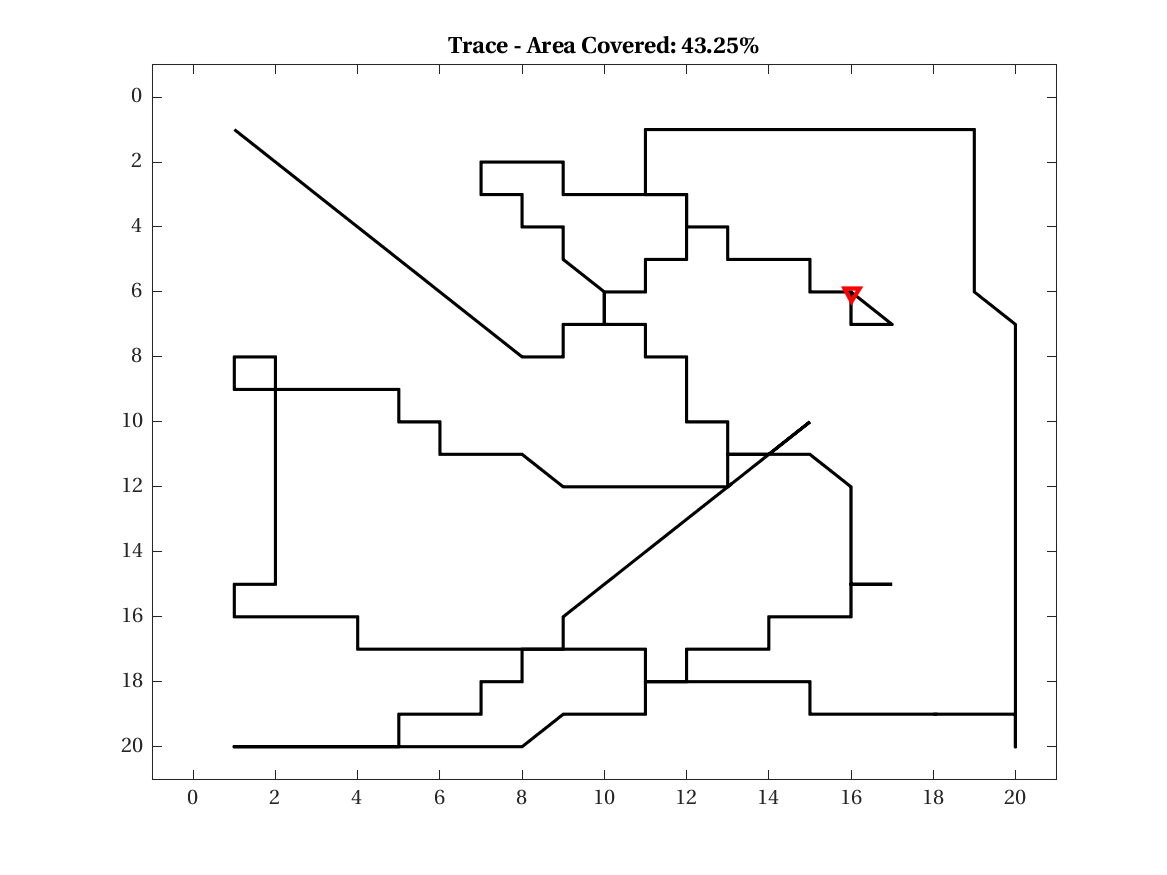
\includegraphics[width=\linewidth]{figures/hbresults/path_mc_40p_20x20_sf_4_seed_2.png}
        \captionsetup{skip=0.20\baselineskip,size=footnotesize}
        \caption{Monte Carlo}
    \end{subfigure}%
    \\
    \begin{subfigure}[t]{0.3333\textwidth}
        \centering
        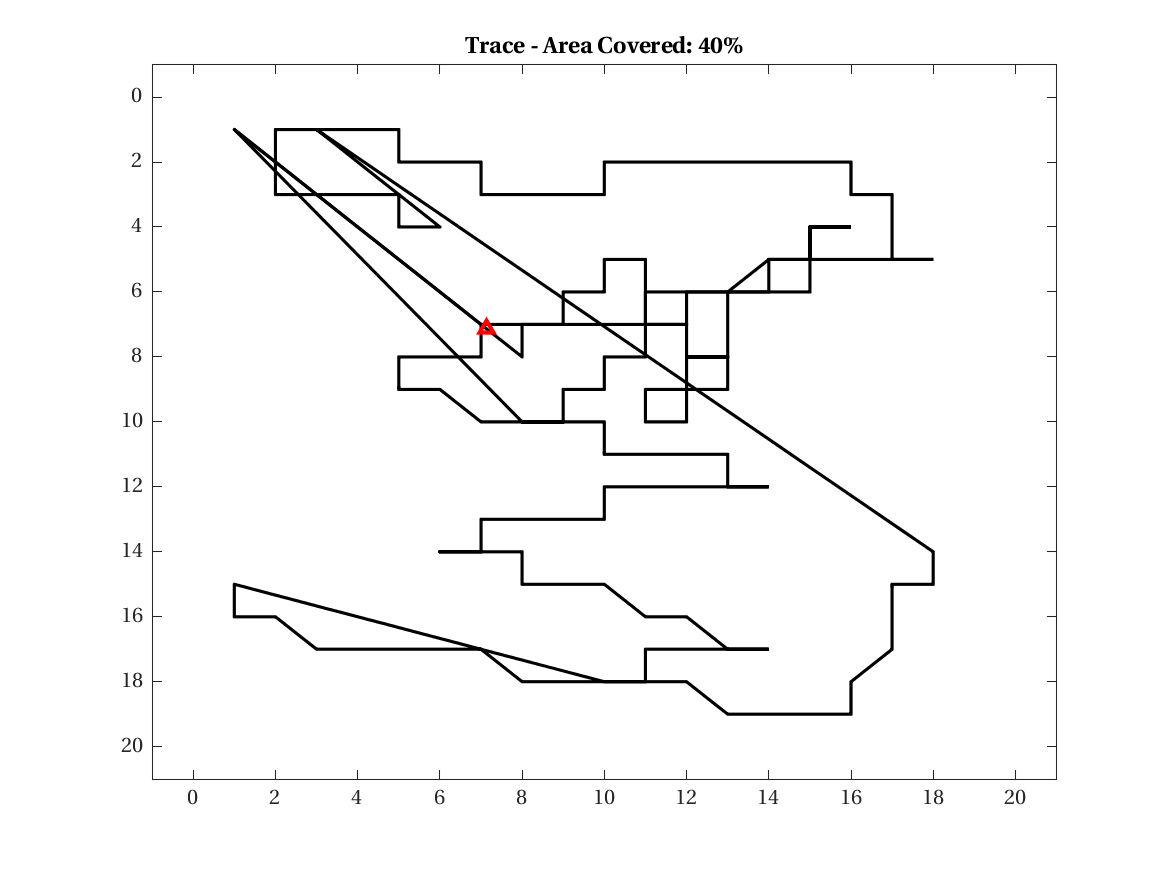
\includegraphics[width=\linewidth]{figures/hbresults/path_nbv_40p_20x20_sf_4_seed_2.png}
        \captionsetup{skip=0.20\baselineskip,size=footnotesize}
        \caption{Greedy NBV}
    \end{subfigure}%
    \begin{subfigure}[t]{0.3333\textwidth}
        \centering
        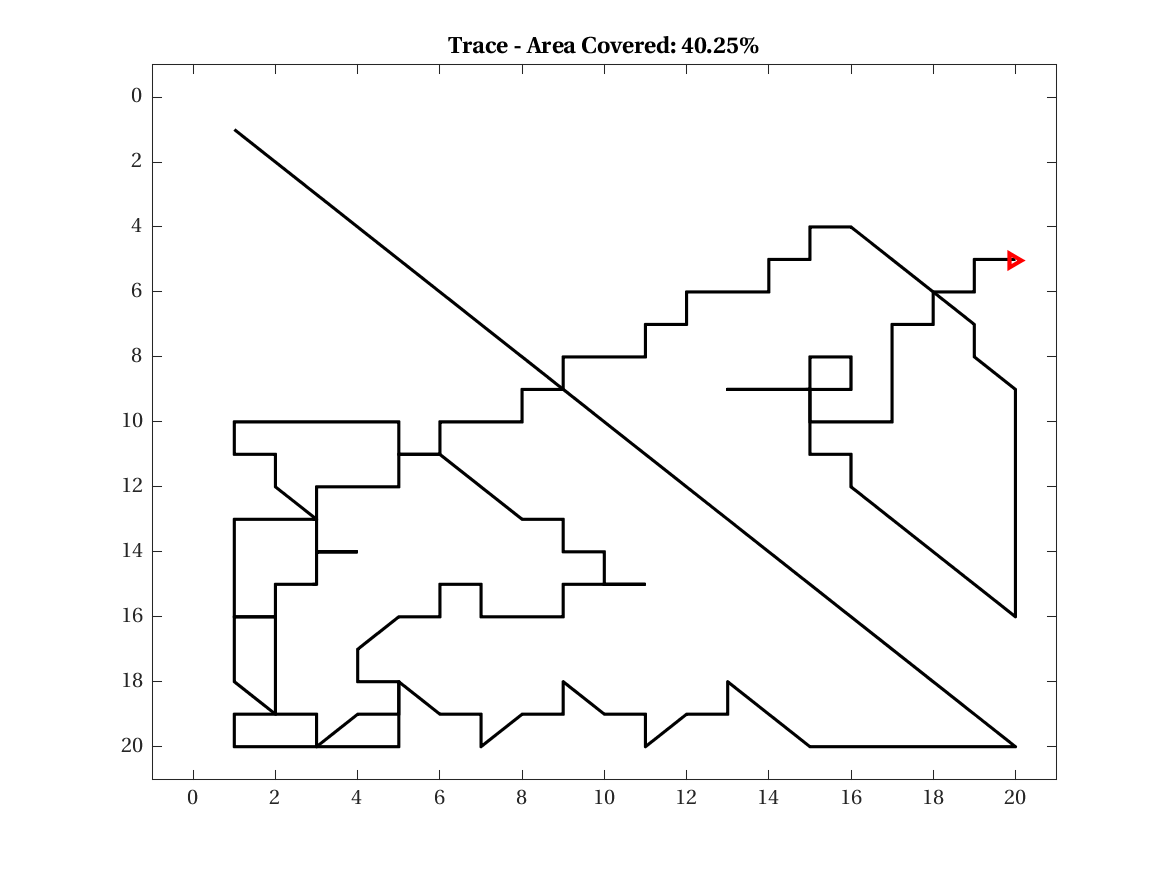
\includegraphics[width=\linewidth]{figures/hbresults/path_gradient_40p_20x20_sf_4_seed_2.png}
        \captionsetup{skip=0.20\baselineskip,size=footnotesize}
        \caption{Gradient Ascent}
    \end{subfigure}%
    \begin{subfigure}[t]{0.3333\textwidth}
        \centering
        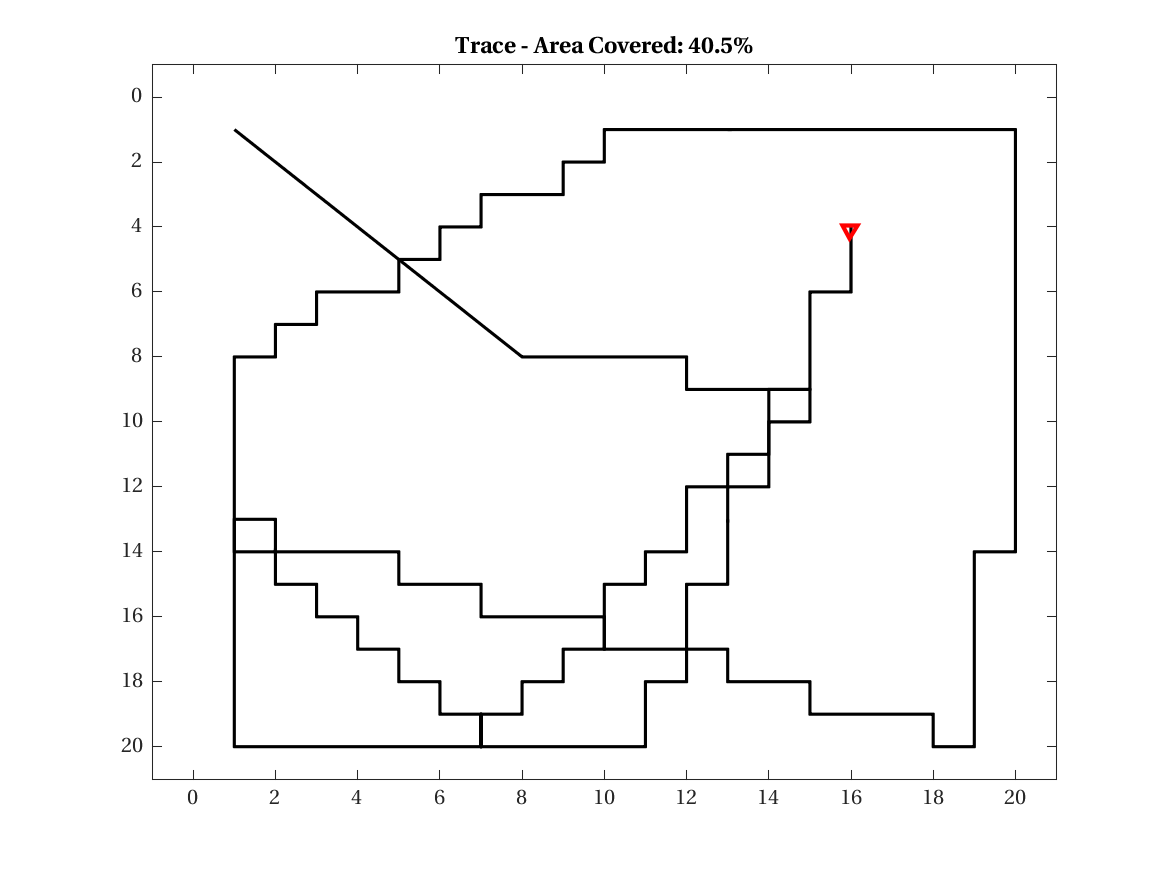
\includegraphics[width=\linewidth]{figures/hbresults/path_gr_40p_20x20_sf_4_seed_2.png}
        \captionsetup{skip=0.20\baselineskip,size=footnotesize}
        \caption{Gradient Range Ascent}
    \end{subfigure}%
    \\
    \begin{subfigure}[t]{0.3333\textwidth}
        \centering
        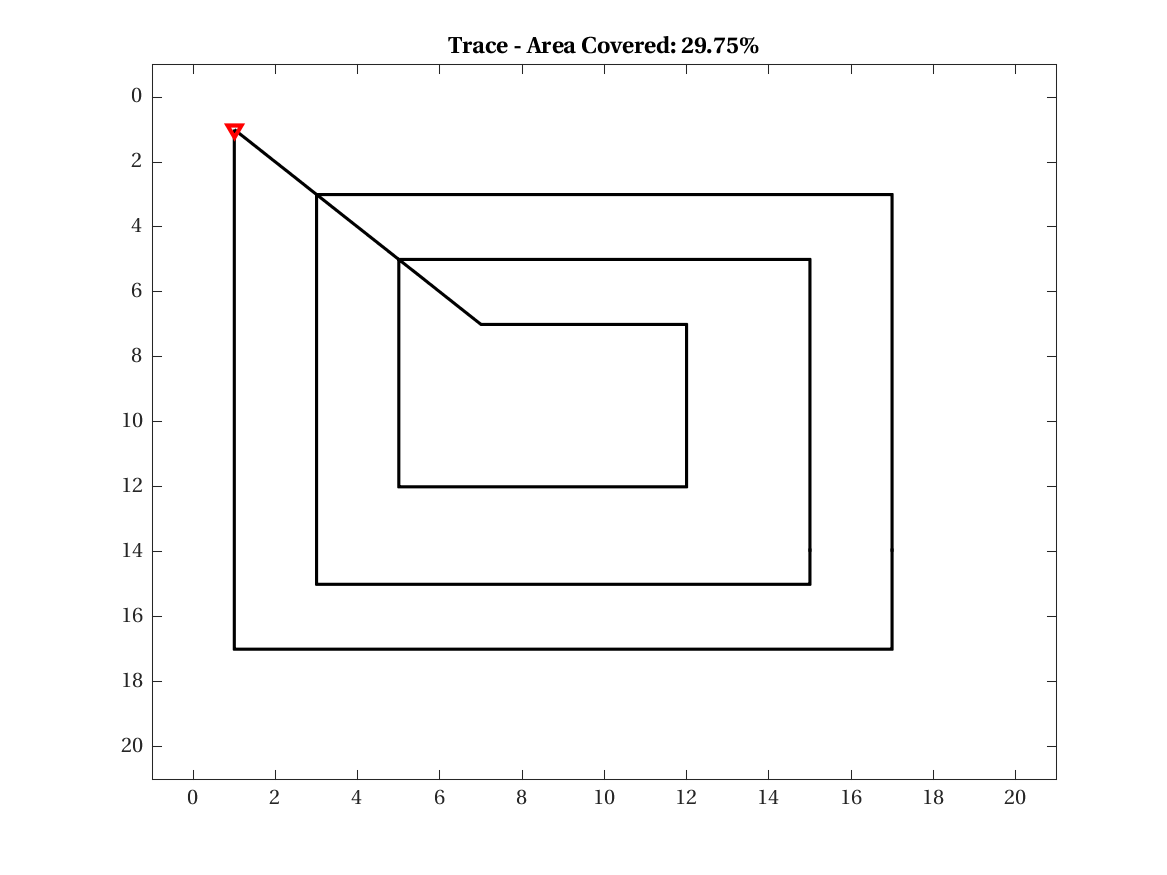
\includegraphics[width=\linewidth]{figures/hbresults/path_zz_40p_20x20_sf_4_seed_2.png}
        \captionsetup{skip=0.20\baselineskip,size=footnotesize}
        \caption{$ZZ_{30}$}
    \end{subfigure}%
    \captionsetup{skip=0.20\baselineskip}
    \caption{Exploration of a field of size $20 \times 20$, $\sigma_{field} = 4$, random seed 2.}
    \label{fig:nbvpathcomp}
\end{figure}

\begin{figure}[htb!]
    \centering
    \begin{subfigure}[t]{0.75\textwidth}
        \centering
        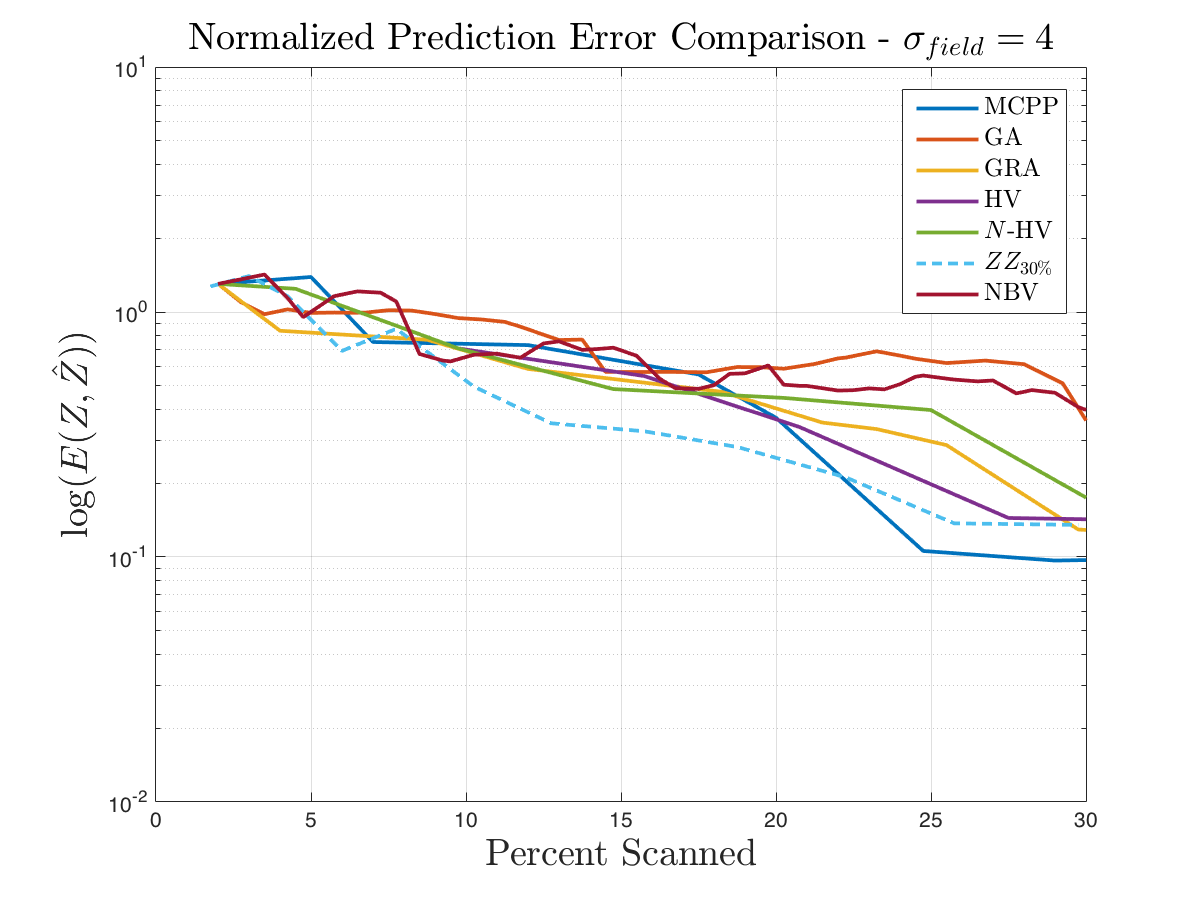
\includegraphics[width=\linewidth]{figures/results/normalized_errors_40p_20x20_sf_4_seed_2_app_10.png}
        \captionsetup{skip=0.20\baselineskip,size=footnotesize}
        \caption{Normalized prediction errors for each method.}
    \end{subfigure}%
    \\
    \begin{subfigure}[t]{0.75\textwidth}
        \centering
        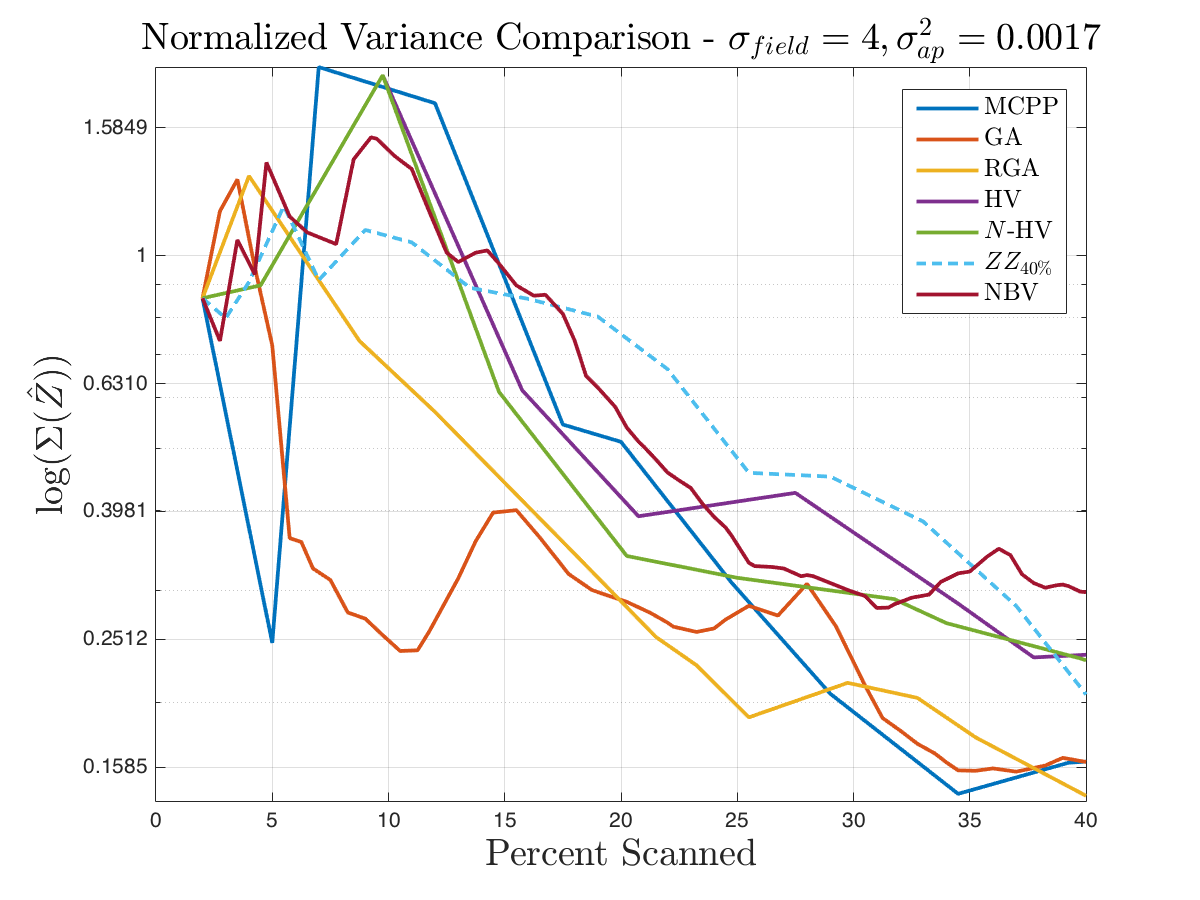
\includegraphics[width=\linewidth]{figures/results/normalized_variances_40p_20x20_sf_4_seed_2_app_10.png}
        \captionsetup{skip=0.20\baselineskip,size=footnotesize}
        \caption{Normalized prediction variances for each method.}
    \end{subfigure}%
    \captionsetup{skip=0.20\baselineskip}
    \caption{Prediction error and variances for an exploration of a field of size $20 \times 20$, $\sigma_{field} = 4$, random seed 2.}
    \label{fig:nbvcomp}
\end{figure}

\FloatBarrier
\clearpage

\section{High Spatial Autocorrelation Results}
The methods will be compared on target fields generated with an autocorrelation factor, $\sigma_{field}$, equal to the field width. A Gaussian filter $G(x,y,100)$ (Equation \ref{eq:gauss_filt}), is convolved with all points on the field.

\begin{figure}[htb!]
    \centering
    \begin{subfigure}[t]{0.3333\textwidth}
        \centering
        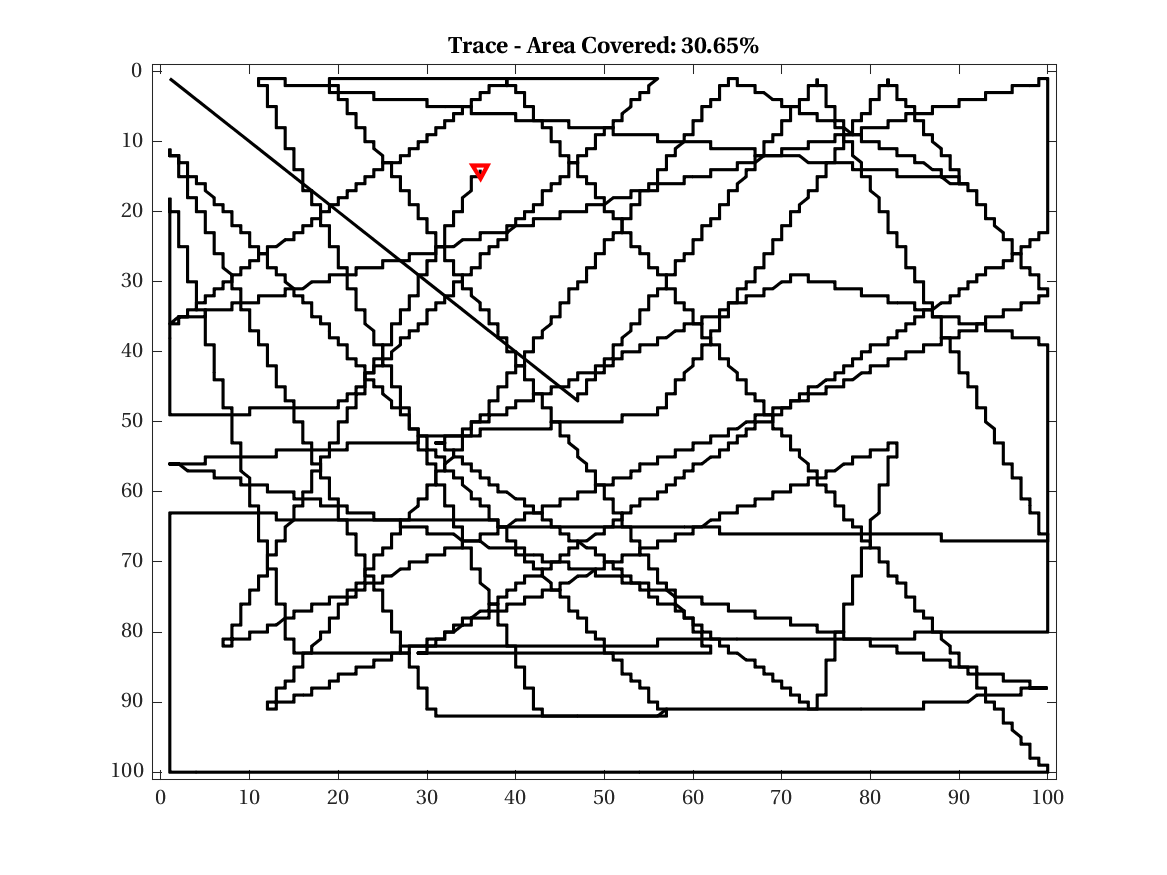
\includegraphics[width=\linewidth]{figures/hbresults/path_nhv_30p_100x100_sf_100_seed_2.png}
        \captionsetup{skip=0.20\baselineskip,size=footnotesize}
        \caption{Highest Variance}
    \end{subfigure}%
    \begin{subfigure}[t]{0.3333\textwidth}
        \centering
        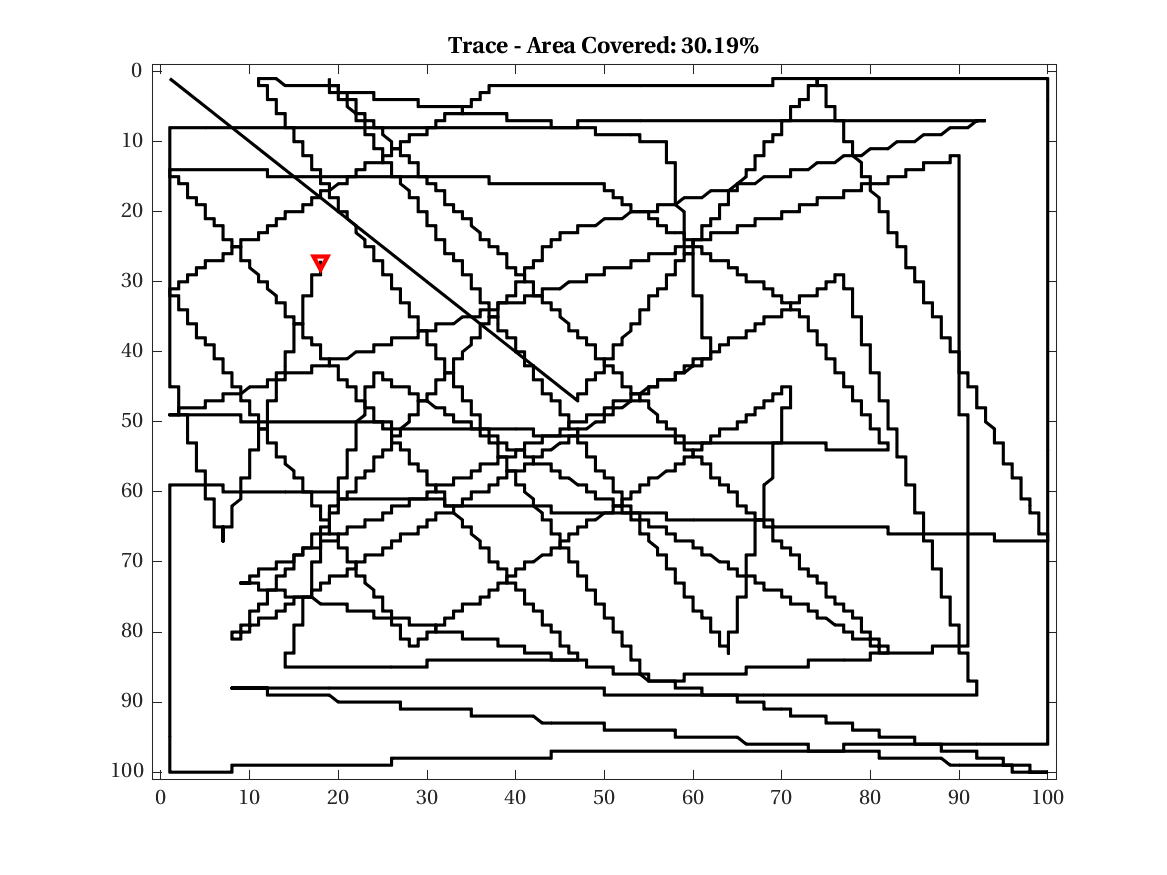
\includegraphics[width=\linewidth]{figures/hbresults/path_nnhv_30p_100x100_sf_100_seed_2.png}
        \captionsetup{skip=0.20\baselineskip,size=footnotesize}
        \caption{$N$ Highest Variance}
    \end{subfigure}%
    \begin{subfigure}[t]{0.3333\textwidth}
        \centering
        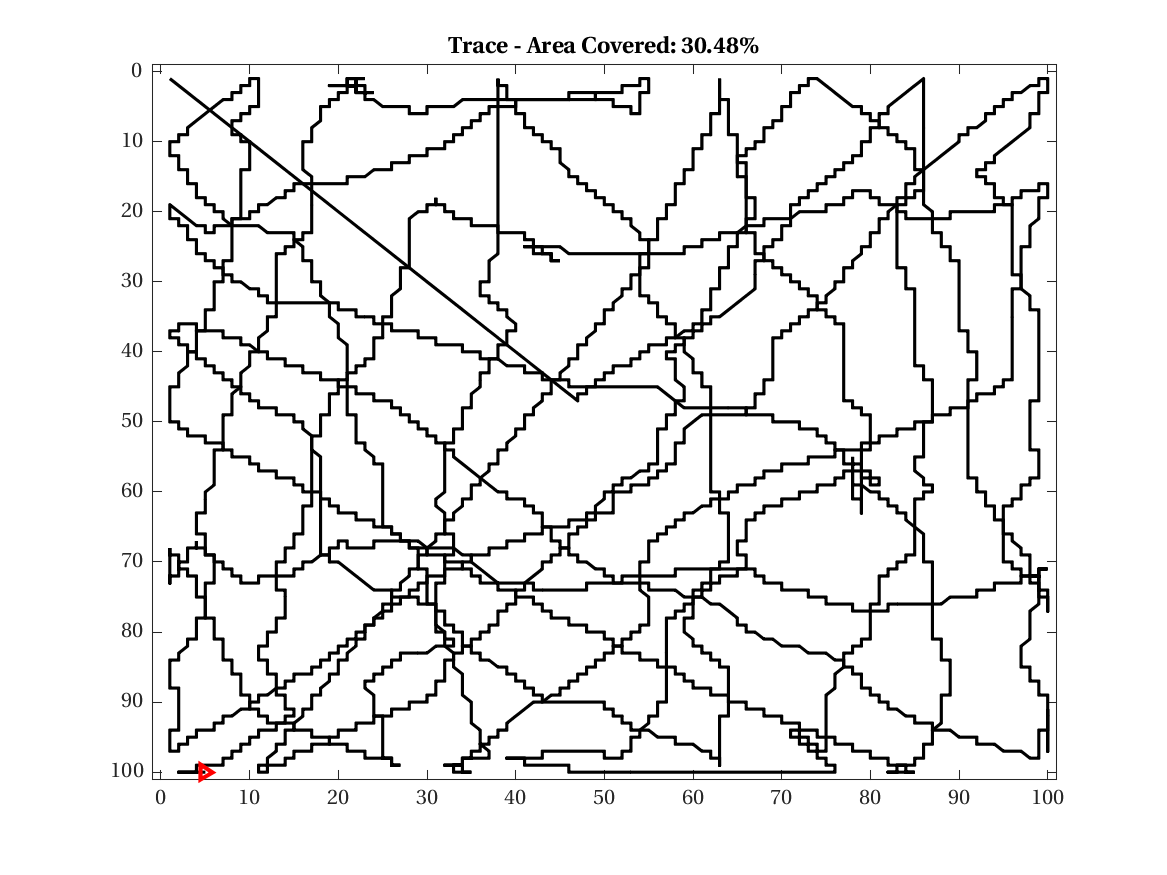
\includegraphics[width=\linewidth]{figures/hbresults/path_mc_30p_100x100_sf_100_seed_2.png}
        \captionsetup{skip=0.20\baselineskip,size=footnotesize}
        \caption{Monte Carlo}
    \end{subfigure}%
    \\
    \begin{subfigure}[t]{0.3333\textwidth}
        \centering
        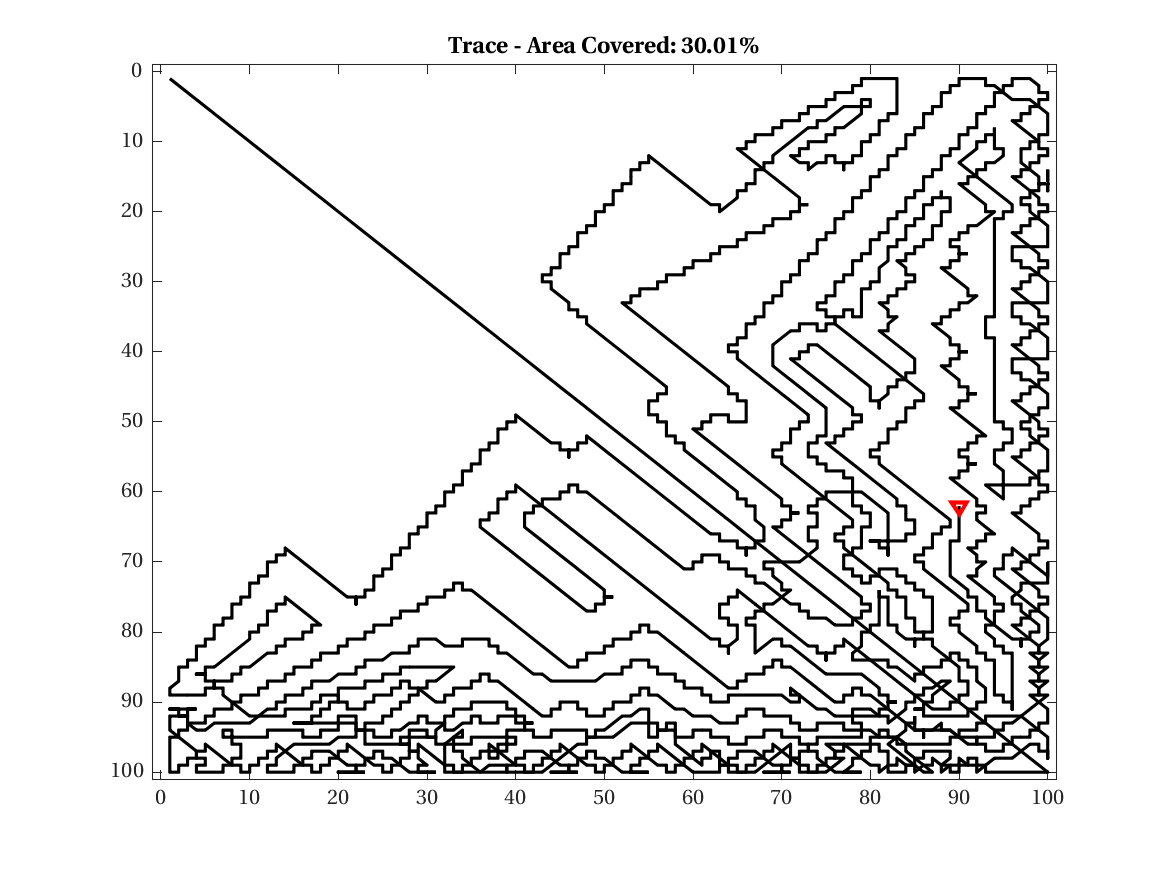
\includegraphics[width=\linewidth]{figures/hbresults/path_gradient_30p_100x100_sf_100_seed_2.png}
        \captionsetup{skip=0.20\baselineskip,size=footnotesize}
        \caption{Gradient Ascent}
    \end{subfigure}%
    \begin{subfigure}[t]{0.3333\textwidth}
        \centering
        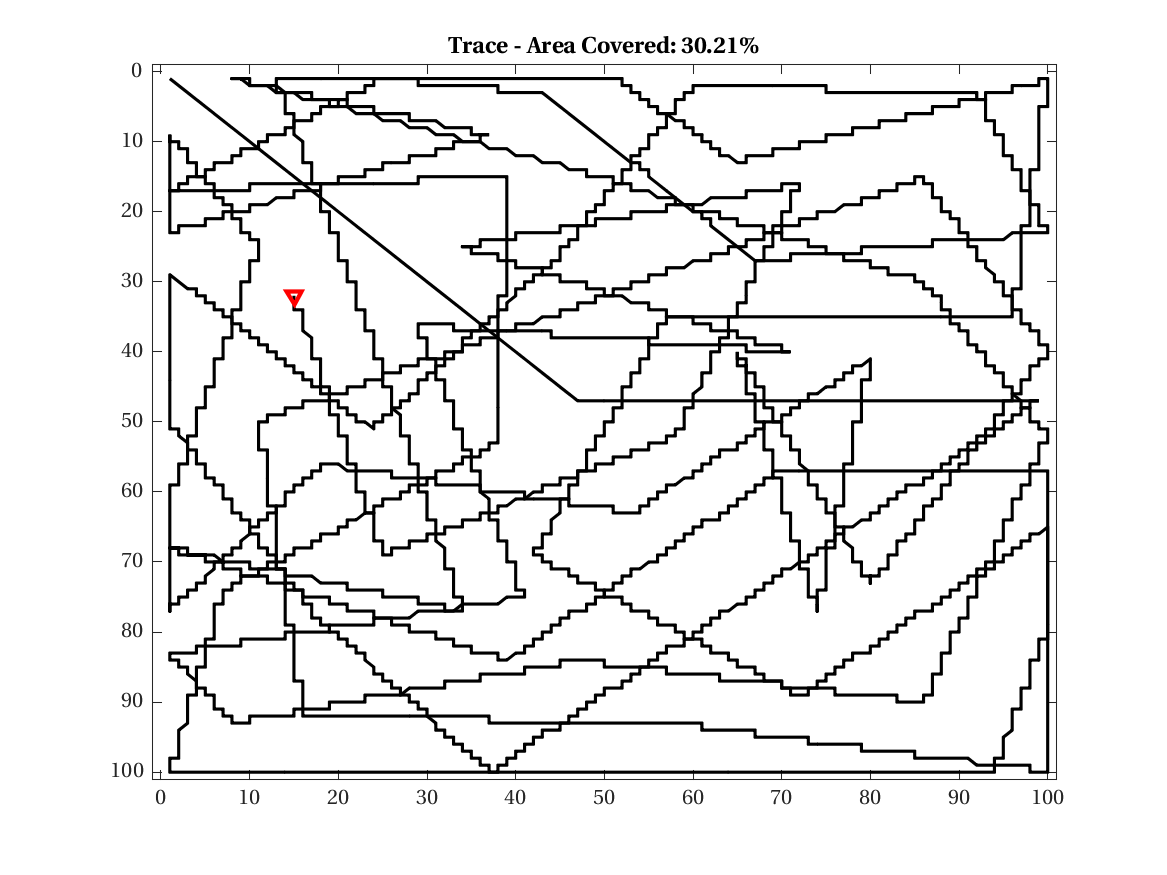
\includegraphics[width=\linewidth]{figures/hbresults/path_gr_30p_100x100_sf_100_seed_2.png}
        \captionsetup{skip=0.20\baselineskip,size=footnotesize}
        \caption{Gradient Range Ascent}
    \end{subfigure}%
    \\
    \begin{subfigure}[t]{0.3333\textwidth}
        \centering
        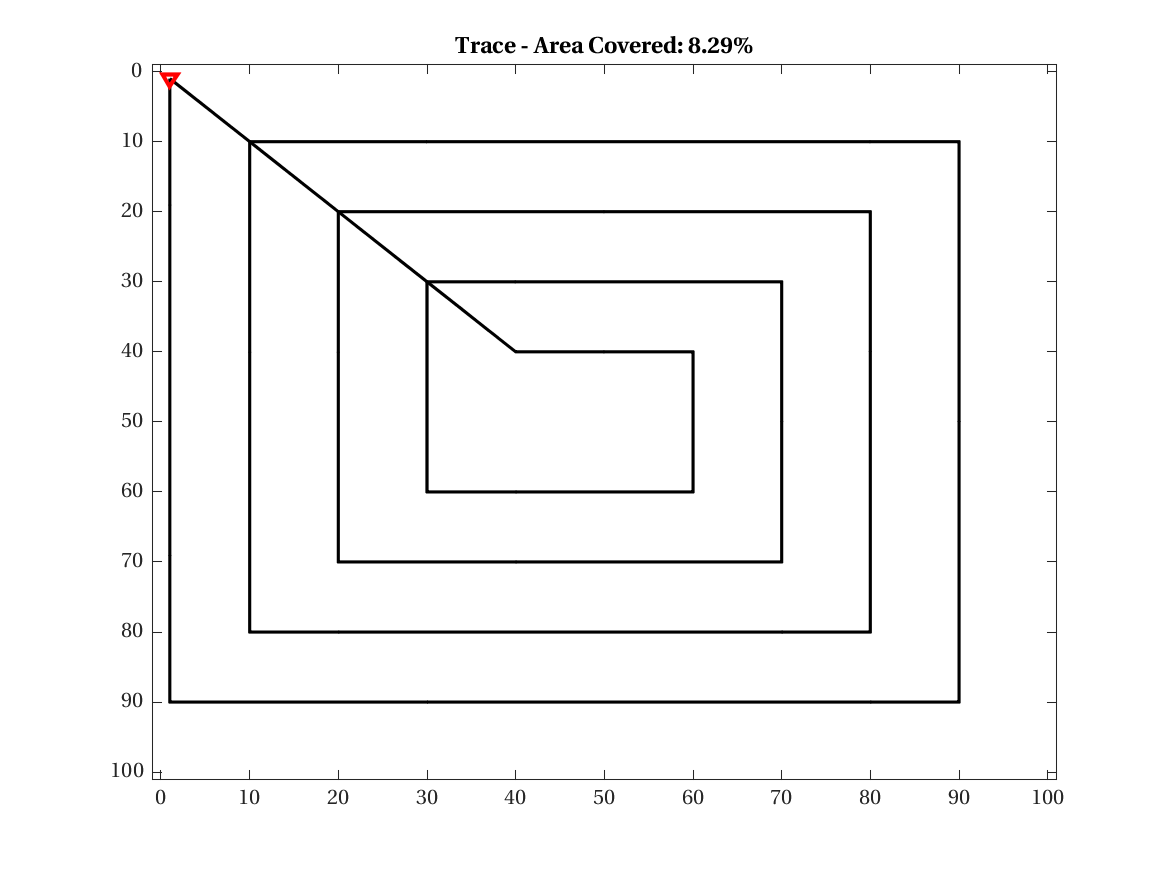
\includegraphics[width=\linewidth]{figures/hbresults/path_zz_10p_100x100_sf_100_seed_2.png}
        \captionsetup{skip=0.20\baselineskip,size=footnotesize}
        \caption{$ZZ_{10}$}
    \end{subfigure}%
    \begin{subfigure}[t]{0.3333\textwidth}
        \centering
        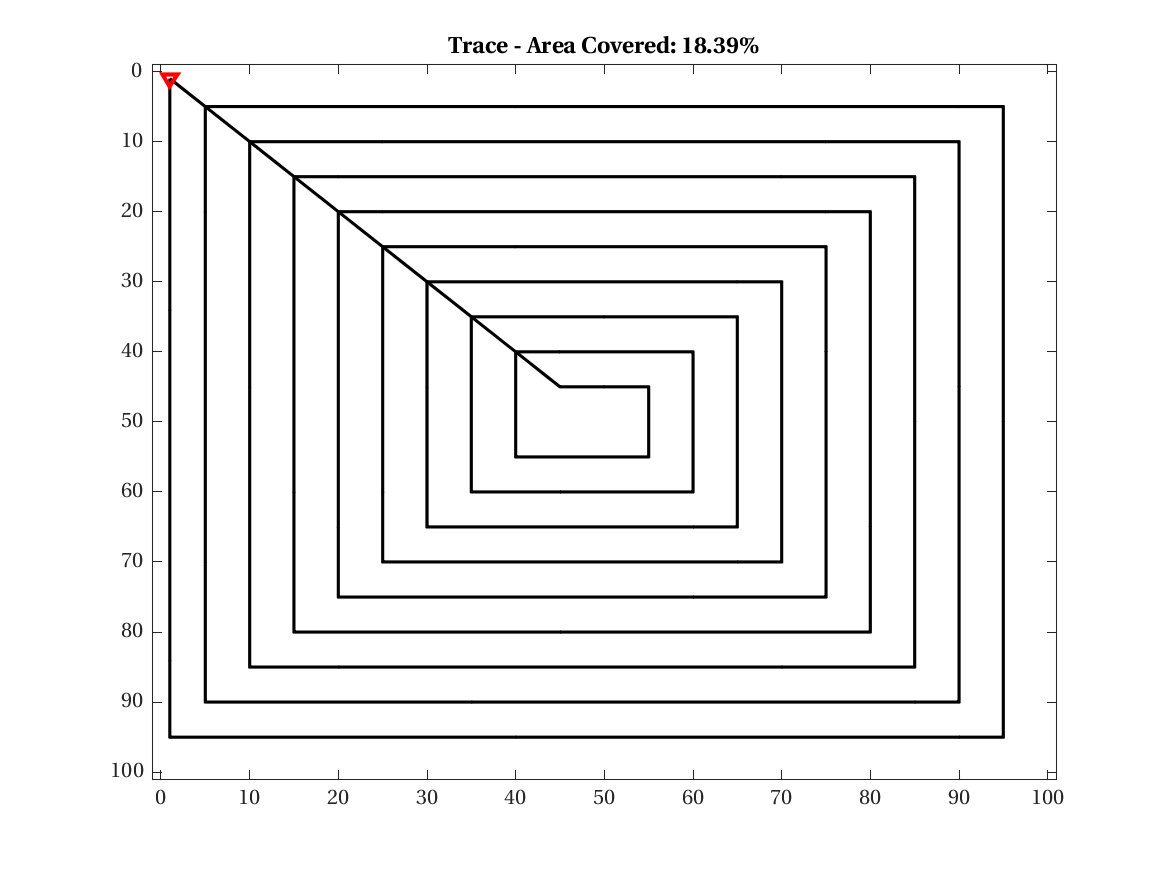
\includegraphics[width=\linewidth]{figures/hbresults/path_zz_20p_100x100_sf_100_seed_2.png}
        \captionsetup{skip=0.20\baselineskip,size=footnotesize}
        \caption{$ZZ_{20}$}
    \end{subfigure}%
    \begin{subfigure}[t]{0.3333\textwidth}
        \centering
        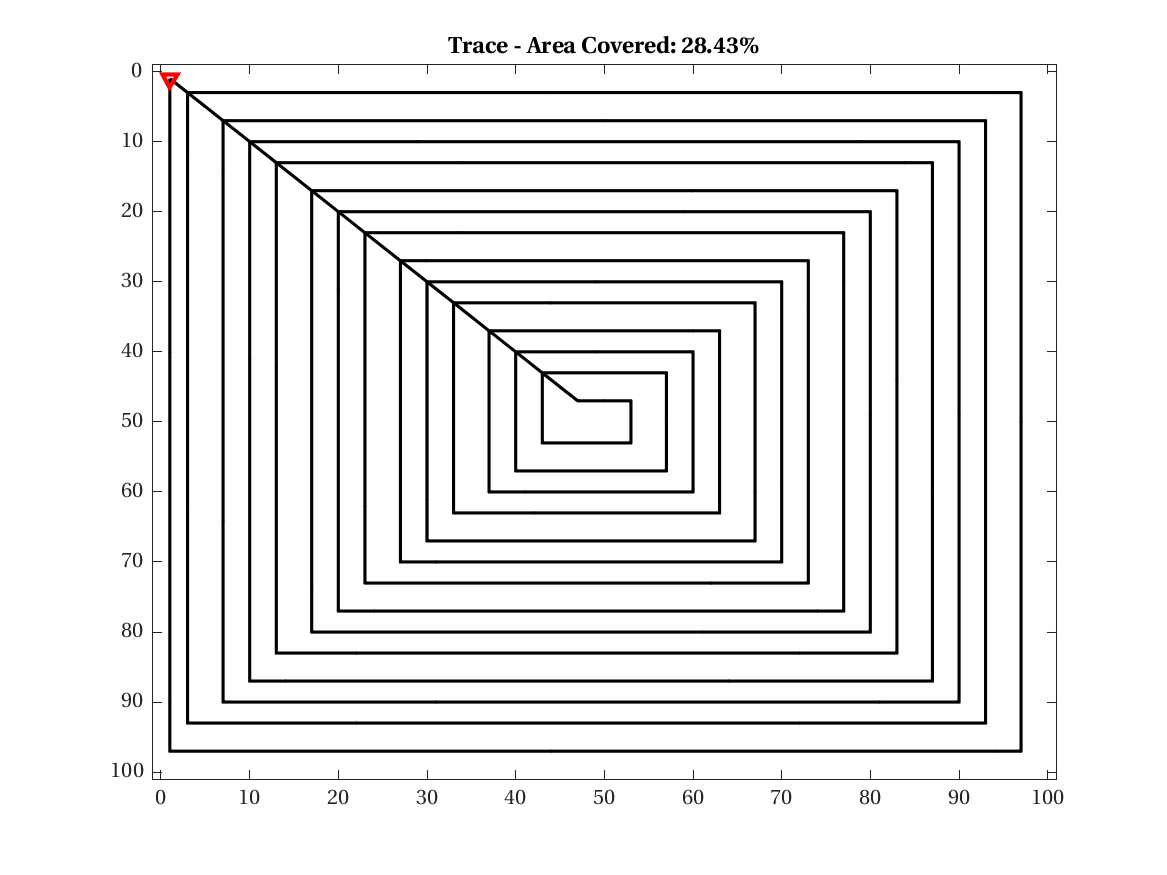
\includegraphics[width=\linewidth]{figures/hbresults/path_zz_30p_100x100_sf_100_seed_2.png}
        \captionsetup{skip=0.20\baselineskip,size=footnotesize}
        \caption{$ZZ_{30}$}
    \end{subfigure}%
    \captionsetup{skip=0.20\baselineskip}
    \caption{Exploration of a field of size $100 \times 100$, $\sigma_{field} = 100$, random seed 2.}
    \label{fig:sf100}
\end{figure}

\begin{figure}[htb!]
    \centering
    \begin{subfigure}[t]{0.75\textwidth}
        \centering
        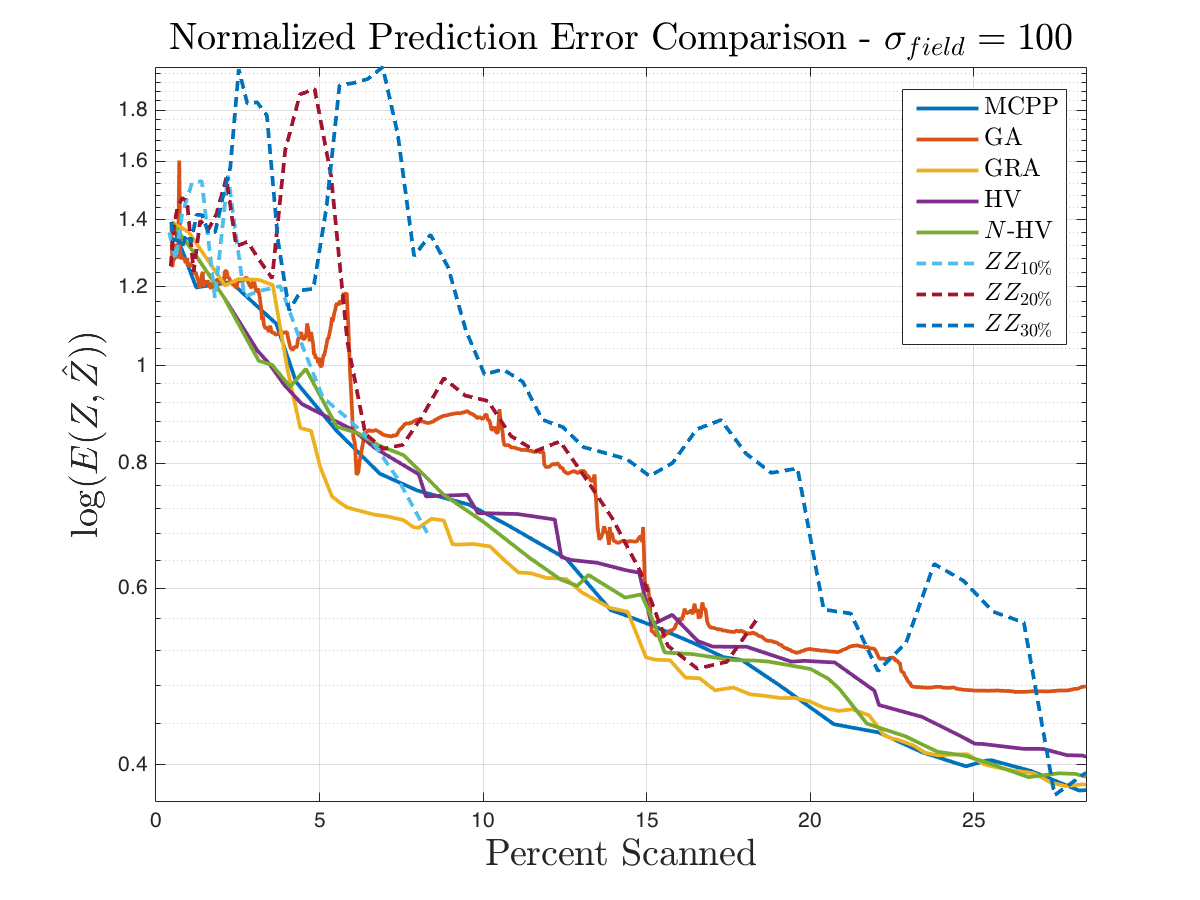
\includegraphics[width=\linewidth]{figures/results/normalized_errors_30p_100x100_sf_100_seed_2_app_50.png}
        \captionsetup{skip=0.20\baselineskip,size=footnotesize}
        \caption{Normalized prediction errors for each method.}
    \end{subfigure}%
    \\
    \begin{subfigure}[t]{0.75\textwidth}
        \centering
        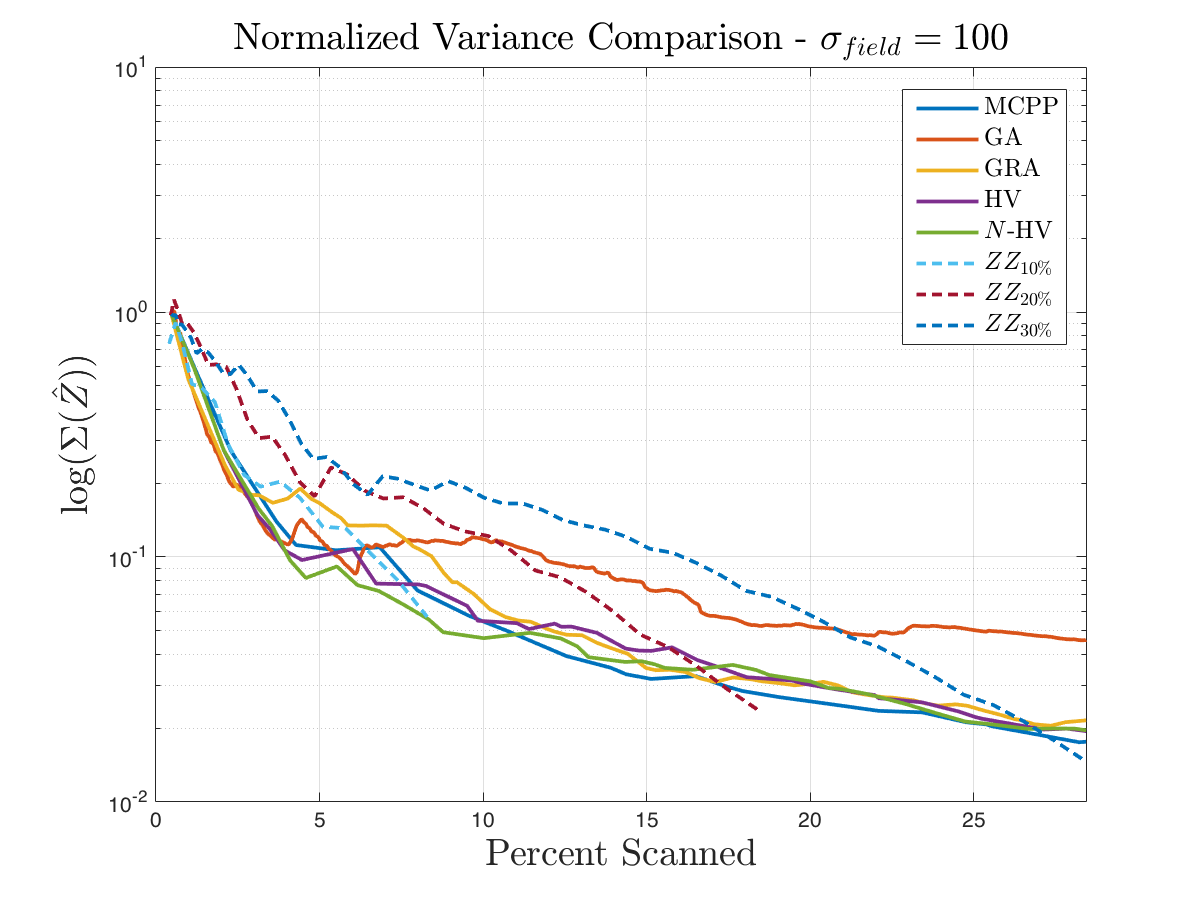
\includegraphics[width=\linewidth]{figures/results/normalized_variances_30p_100x100_sf_100_seed_2_app_50.png}
        \captionsetup{skip=0.20\baselineskip,size=footnotesize}
        \caption{Normalized prediction variances for each method.}
    \end{subfigure}%
    \captionsetup{skip=0.20\baselineskip}
    \caption{Prediction error and variances for an exploration of a field of size $100 \times 100$, $\sigma_{field} = 100$, random seed 2.}
    \label{fig:errvar100}
\end{figure}

\FloatBarrier
\clearpage

\section{Half Width Spatial Autocorrelation Results}
The methods will be compared on target fields generated with an autocorrelation factor, $\sigma_{field}$, equal to the half of the target field's width. A Gaussian filter $G(x,y,50)$ (Equation \ref{eq:gauss_filt}), is convolved with all points on the field.

\begin{figure}[htb!]
    \centering
    \begin{subfigure}[t]{0.3333\textwidth}
        \centering
        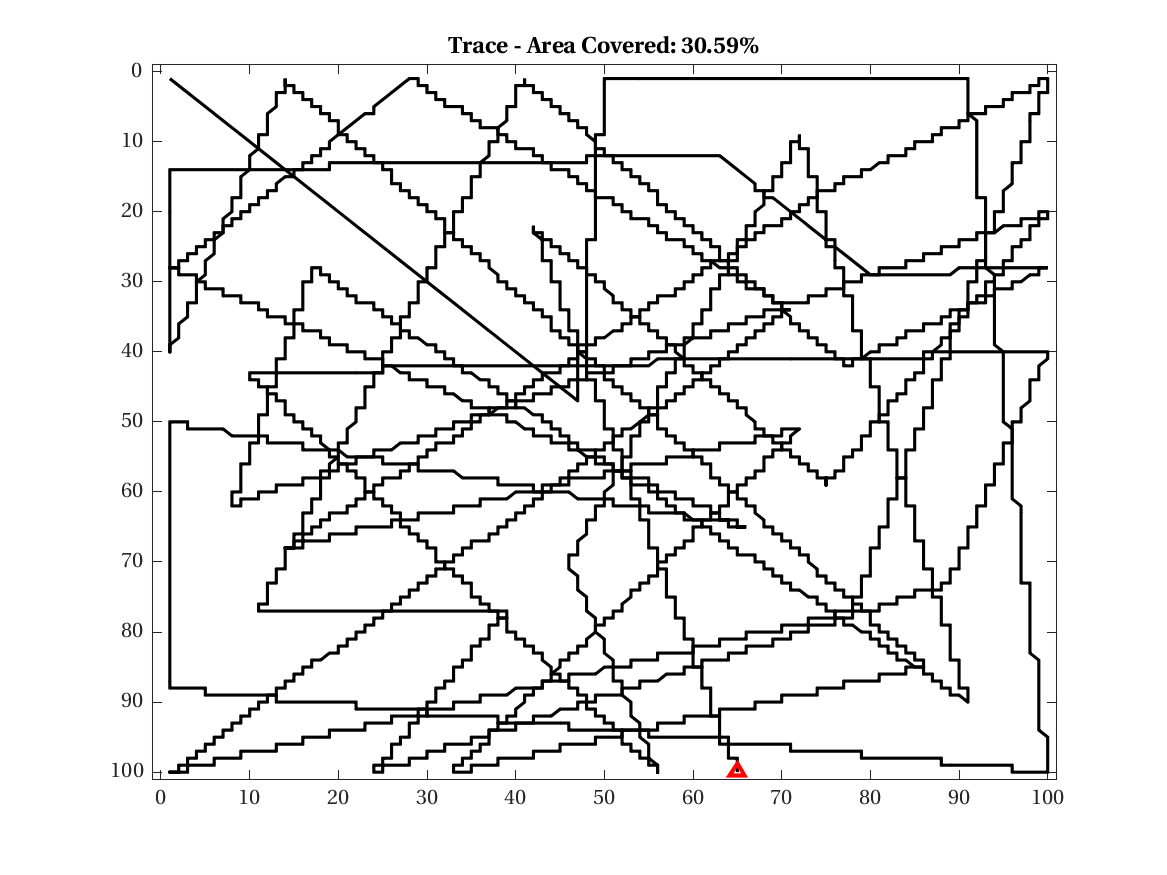
\includegraphics[width=\linewidth]{figures/hbresults/path_nhv_30p_100x100_sf_50_seed_2.png}
        \captionsetup{skip=0.20\baselineskip,size=footnotesize}
        \caption{Highest Variance}
    \end{subfigure}%
    \begin{subfigure}[t]{0.3333\textwidth}
        \centering
        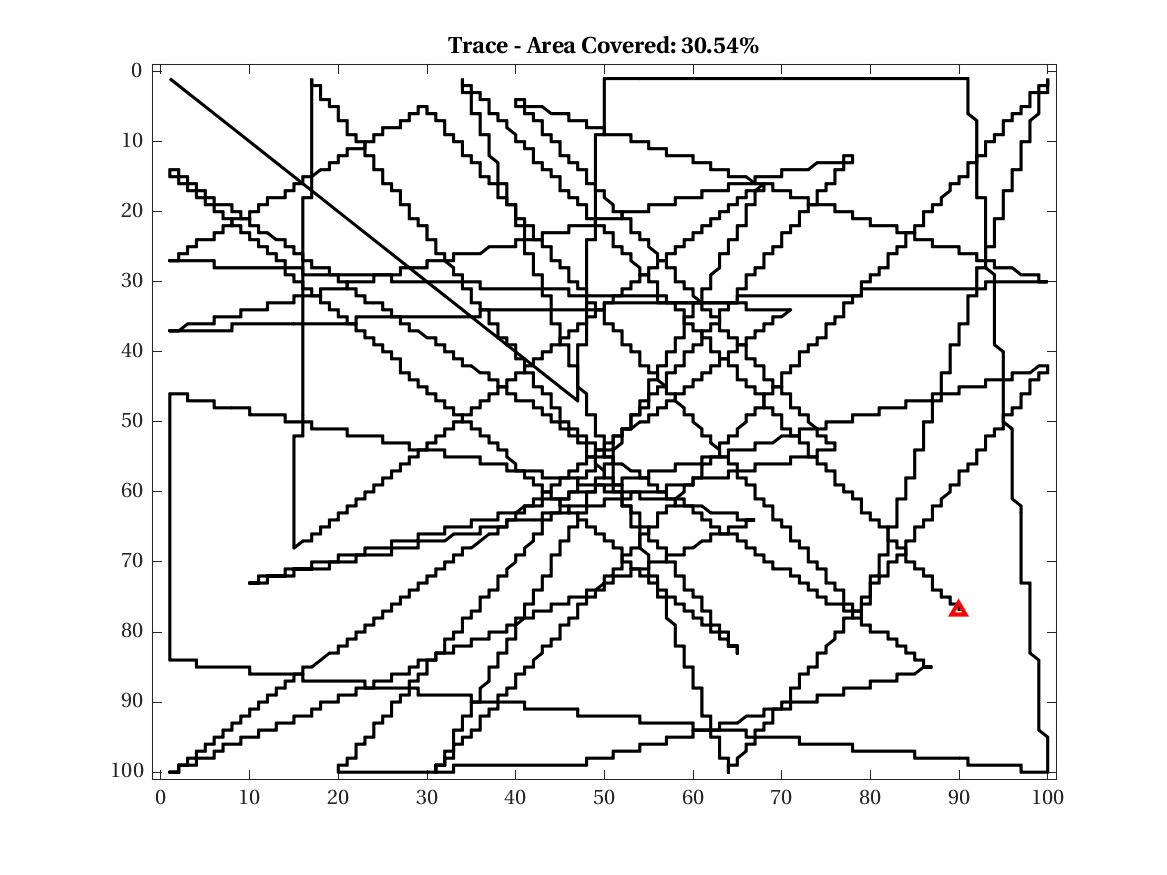
\includegraphics[width=\linewidth]{figures/hbresults/path_nnhv_30p_100x100_sf_50_seed_2.png}
        \captionsetup{skip=0.20\baselineskip,size=footnotesize}
        \caption{$N$ Highest Variance}
    \end{subfigure}%
    \begin{subfigure}[t]{0.3333\textwidth}
        \centering
        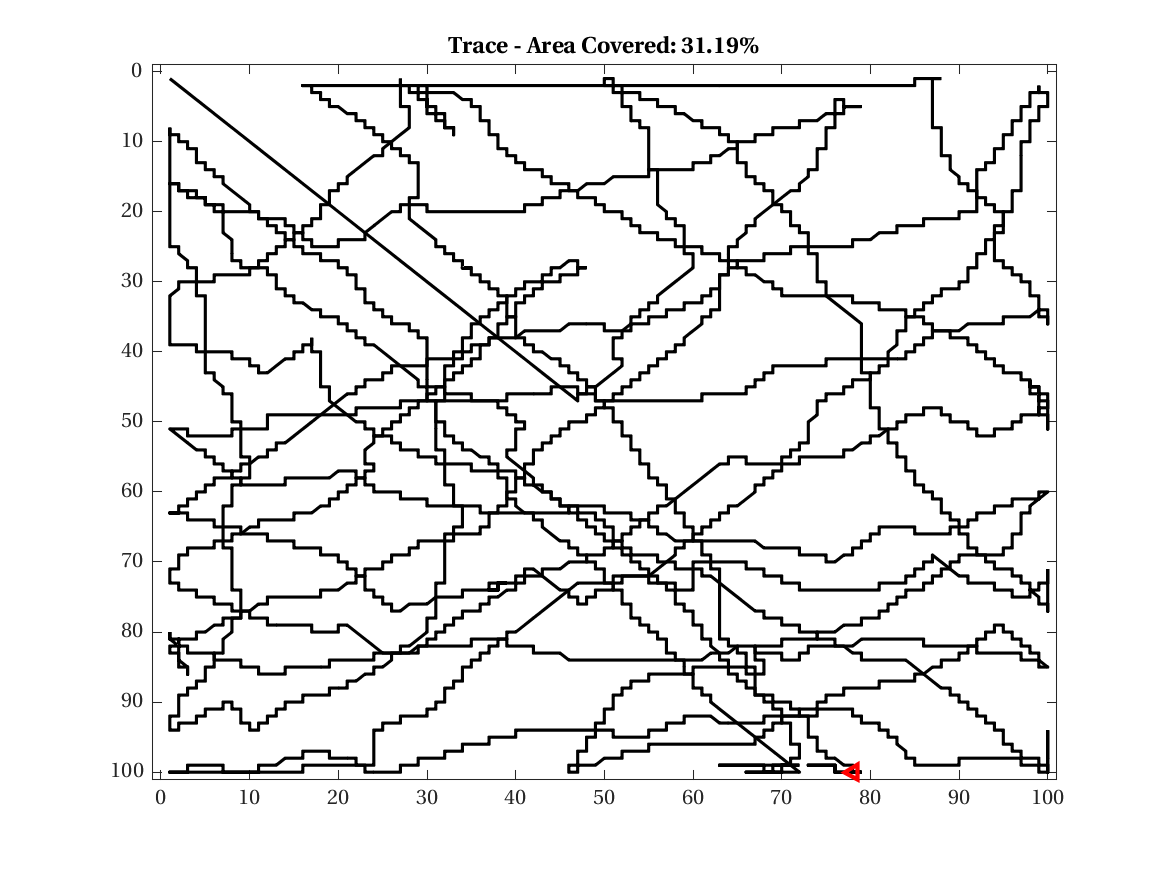
\includegraphics[width=\linewidth]{figures/hbresults/path_mc_30p_100x100_sf_50_seed_2.png}
        \captionsetup{skip=0.20\baselineskip,size=footnotesize}
        \caption{Monte Carlo}
    \end{subfigure}%
    \\
    \begin{subfigure}[t]{0.3333\textwidth}
        \centering
        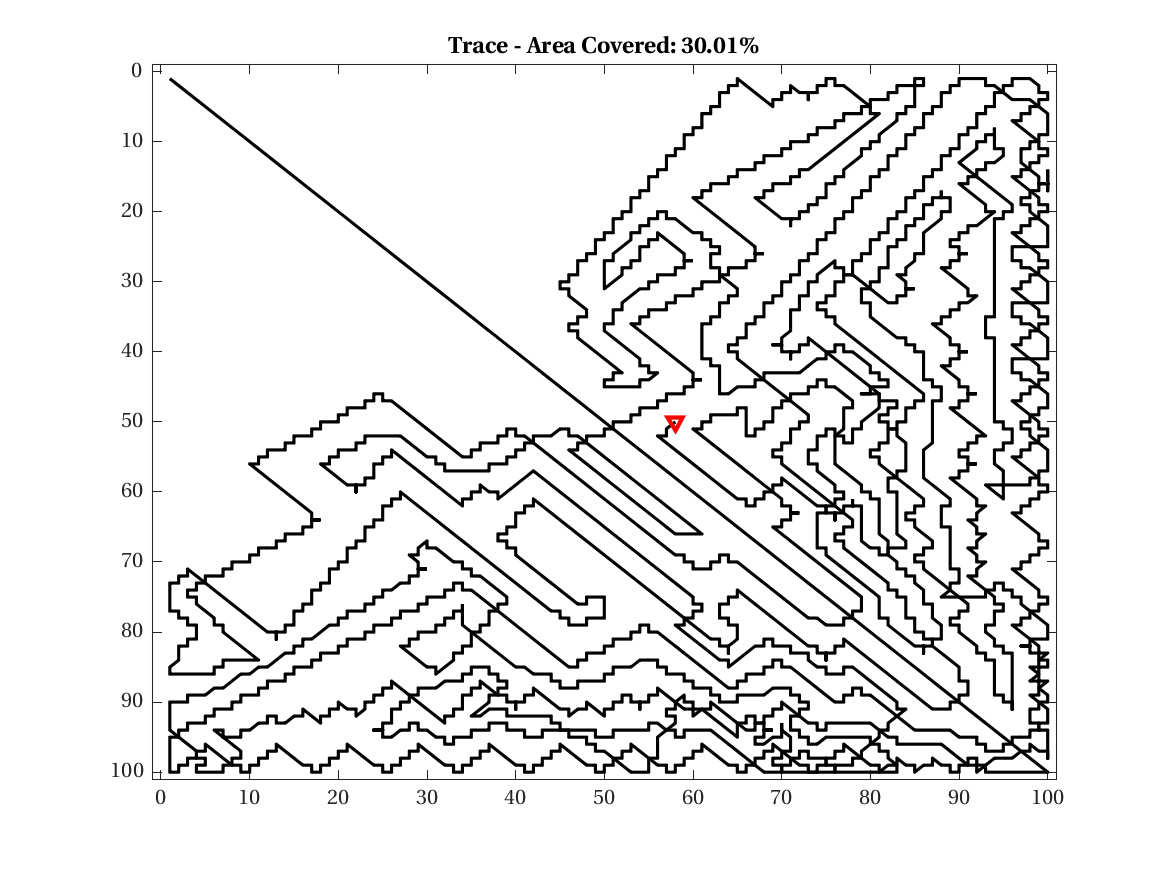
\includegraphics[width=\linewidth]{figures/hbresults/path_gradient_30p_100x100_sf_50_seed_2.png}
        \captionsetup{skip=0.20\baselineskip,size=footnotesize}
        \caption{Gradient Ascent}
    \end{subfigure}%
    \begin{subfigure}[t]{0.3333\textwidth}
        \centering
        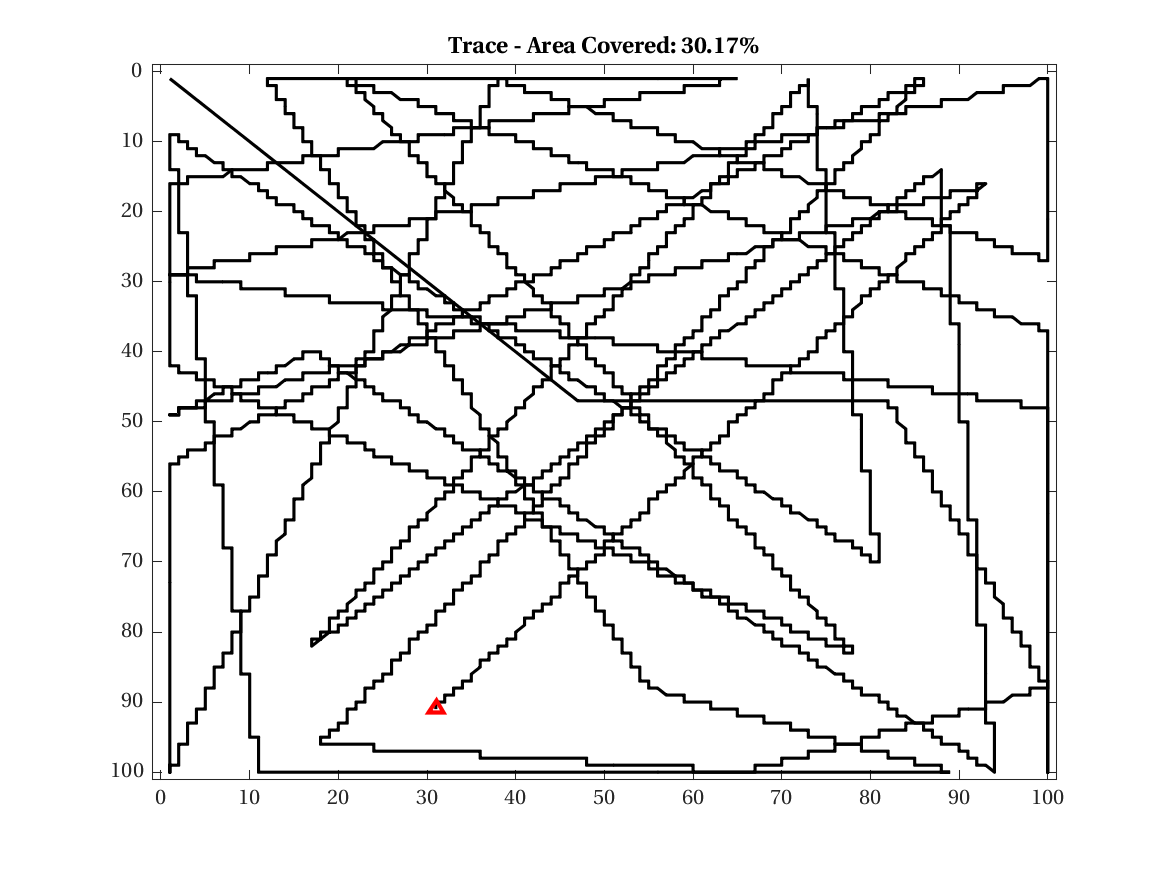
\includegraphics[width=\linewidth]{figures/hbresults/path_gr_30p_100x100_sf_50_seed_2.png}
        \captionsetup{skip=0.20\baselineskip,size=footnotesize}
        \caption{Gradient Range Ascent}
    \end{subfigure}%
    \\
    \begin{subfigure}[t]{0.3333\textwidth}
        \centering
        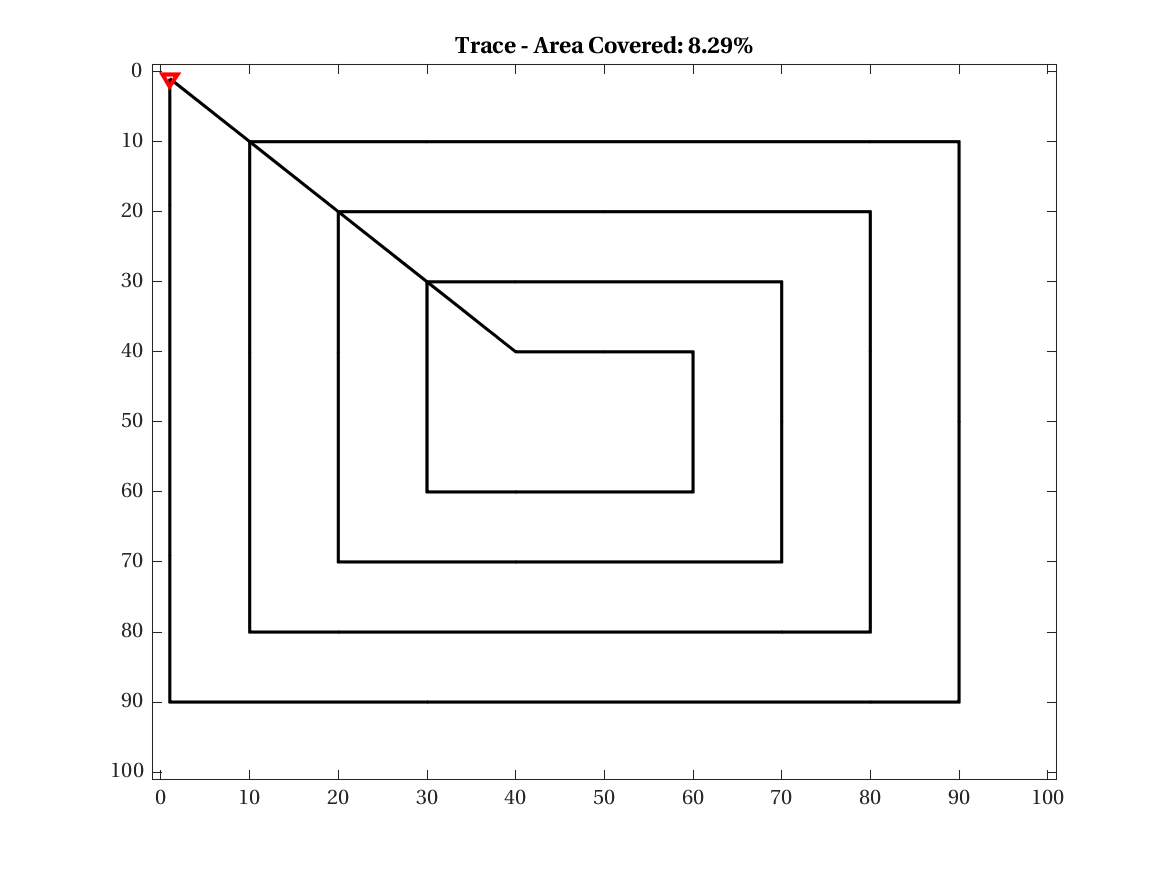
\includegraphics[width=\linewidth]{figures/hbresults/path_zz_10p_100x100_sf_50_seed_2.png}
        \captionsetup{skip=0.20\baselineskip,size=footnotesize}
        \caption{$ZZ_{10}$}
    \end{subfigure}%
    \begin{subfigure}[t]{0.3333\textwidth}
        \centering
        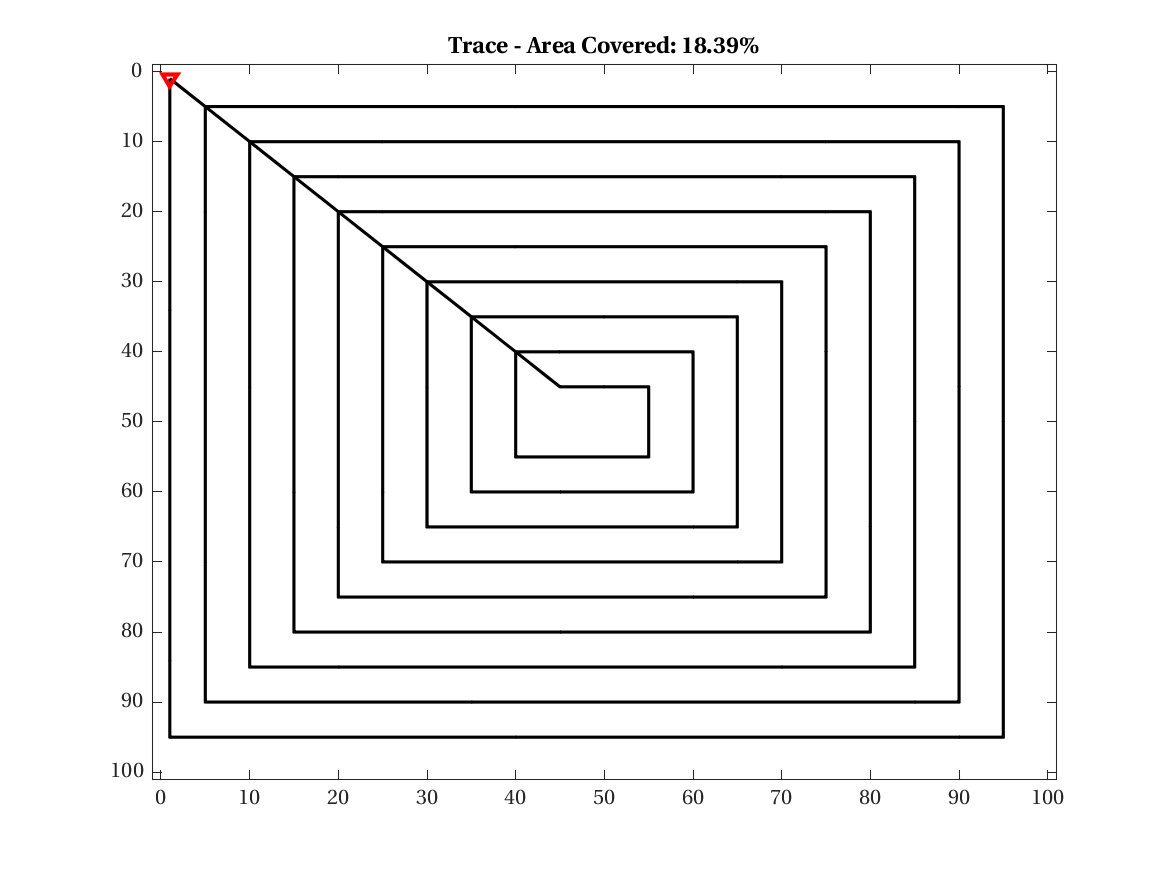
\includegraphics[width=\linewidth]{figures/hbresults/path_zz_20p_100x100_sf_50_seed_2.png}
        \captionsetup{skip=0.20\baselineskip,size=footnotesize}
        \caption{$ZZ_{20}$}
    \end{subfigure}%
    \begin{subfigure}[t]{0.3333\textwidth}
        \centering
        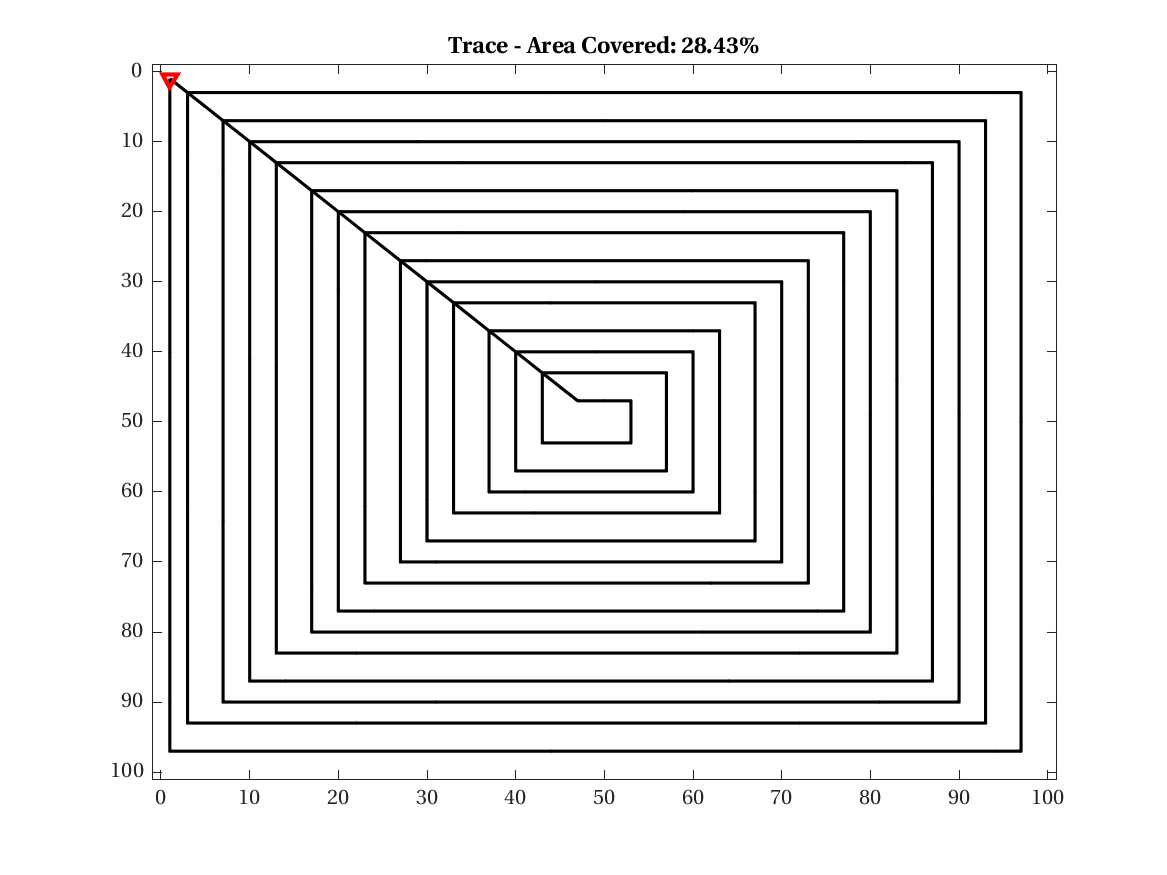
\includegraphics[width=\linewidth]{figures/hbresults/path_zz_30p_100x100_sf_50_seed_2.png}
        \captionsetup{skip=0.20\baselineskip,size=footnotesize}
        \caption{$ZZ_{30}$}
    \end{subfigure}%
    \captionsetup{skip=0.20\baselineskip}
    \caption{Exploration of a field of size $100 \times 100$, $\sigma_{field} = \frac{w}{2} = 50$, random seed 2.}
    \label{fig:sf50}
\end{figure}

\begin{figure}[htb!]
    \centering
    \begin{subfigure}[t]{0.75\textwidth}
        \centering
        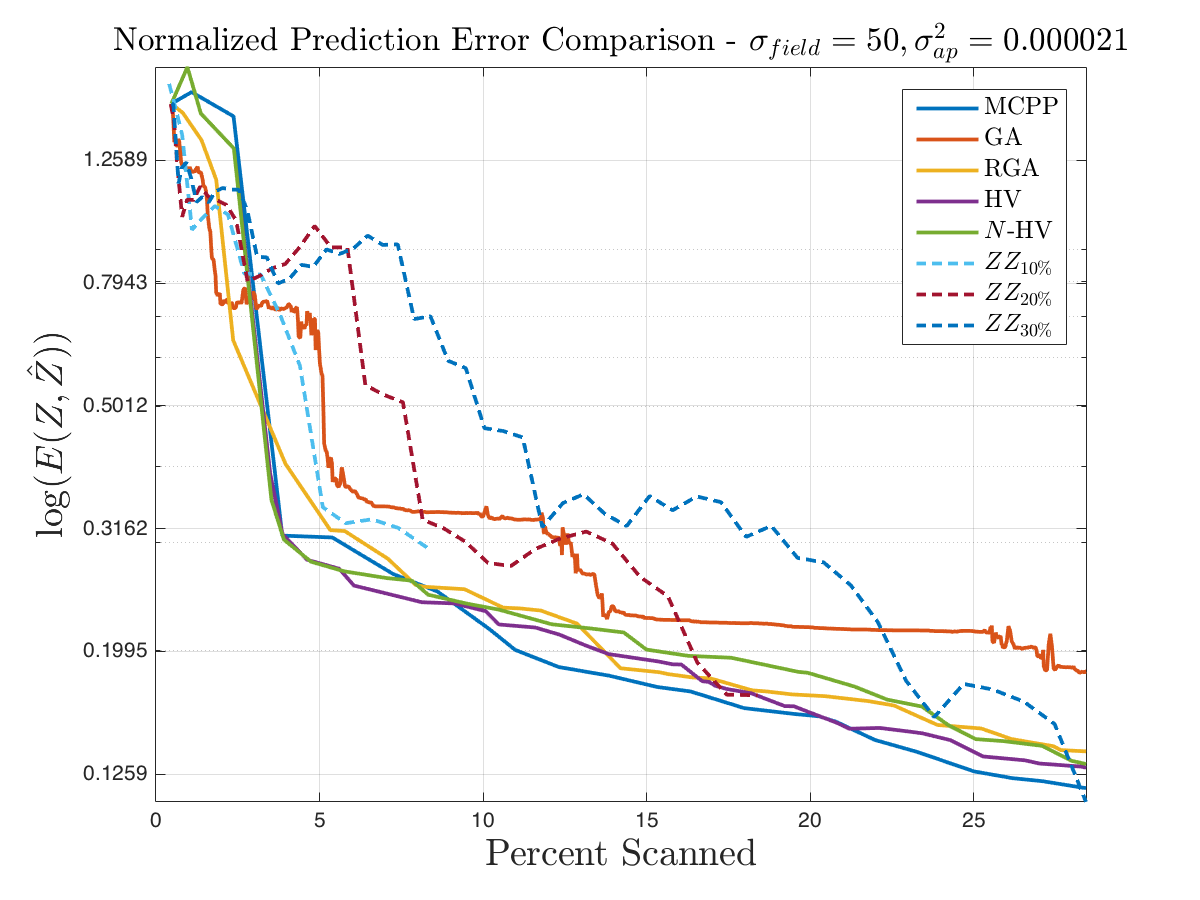
\includegraphics[width=\linewidth]{figures/results/normalized_errors_30p_100x100_sf_50_seed_2_app_50.png}
        \captionsetup{skip=0.20\baselineskip,size=footnotesize}
        \caption{Normalized prediction errors for each method.}
    \end{subfigure}%
    \\
    \begin{subfigure}[t]{0.75\textwidth}
        \centering
        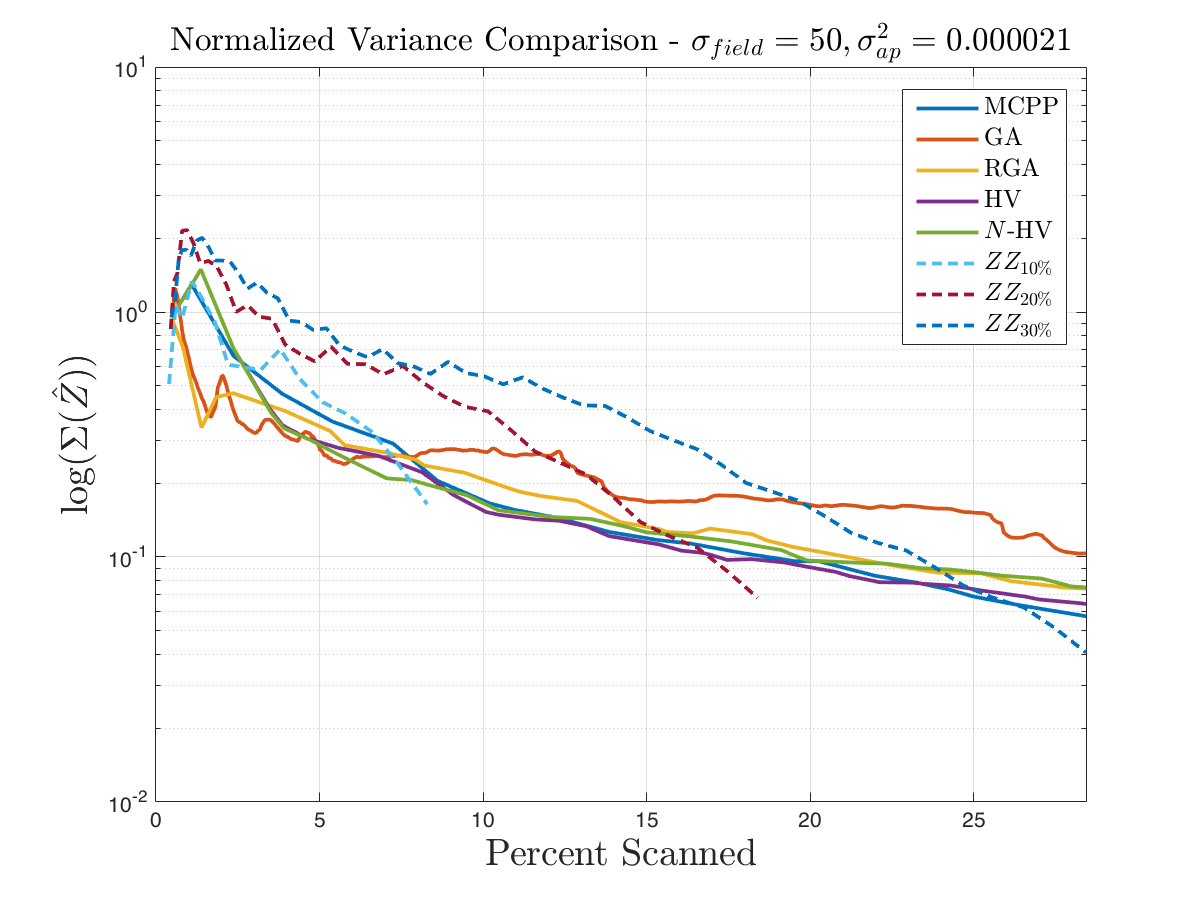
\includegraphics[width=\linewidth]{figures/results/normalized_variances_30p_100x100_sf_50_seed_2_app_50.png}
        \captionsetup{skip=0.20\baselineskip,size=footnotesize}
        \caption{Normalized prediction variances for each method.}
    \end{subfigure}%
    \captionsetup{skip=0.20\baselineskip}
    \caption{Prediction error and variances for an exploration of a field of size $100 \times 100$, $\sigma_{field} = 50$, random seed 2.}
    \label{fig:errvar50}
\end{figure}

\FloatBarrier
\clearpage

\section{Low Spatial Autocorrelation Results}
The methods will be compared on target fields generated with an autocorrelation factor, $\sigma_{field}$, equal to one. A Gaussian filter $G(x,y,1)$ (Equation \ref{eq:gauss_filt}), is convolved with all points on the field.

\begin{figure}[htb!]
    \centering
    \begin{subfigure}[t]{0.3333\textwidth}
        \centering
        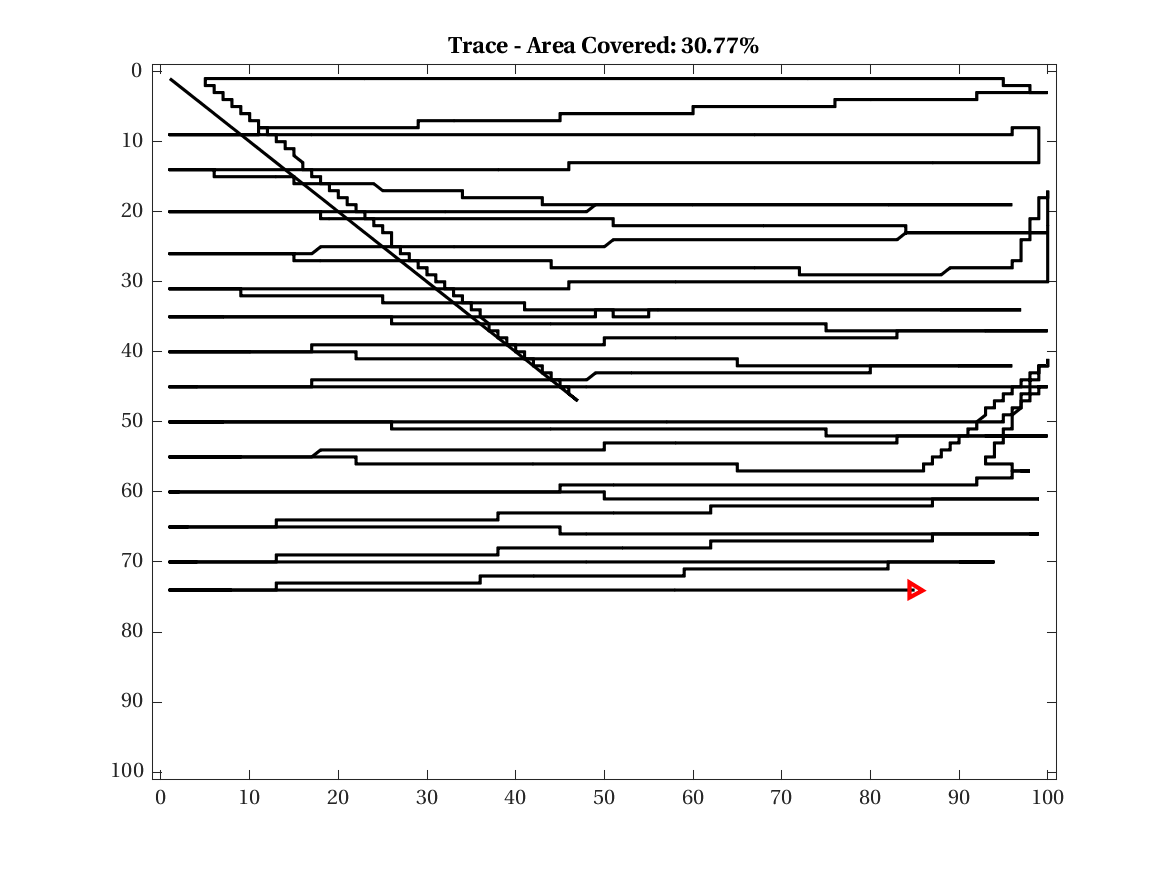
\includegraphics[width=\linewidth]{figures/hbresults/path_nhv_30p_100x100_sf_1_seed_2.png}
        \captionsetup{skip=0.20\baselineskip,size=footnotesize}
        \caption{Highest Variance}
    \end{subfigure}%
    \begin{subfigure}[t]{0.3333\textwidth}
        \centering
        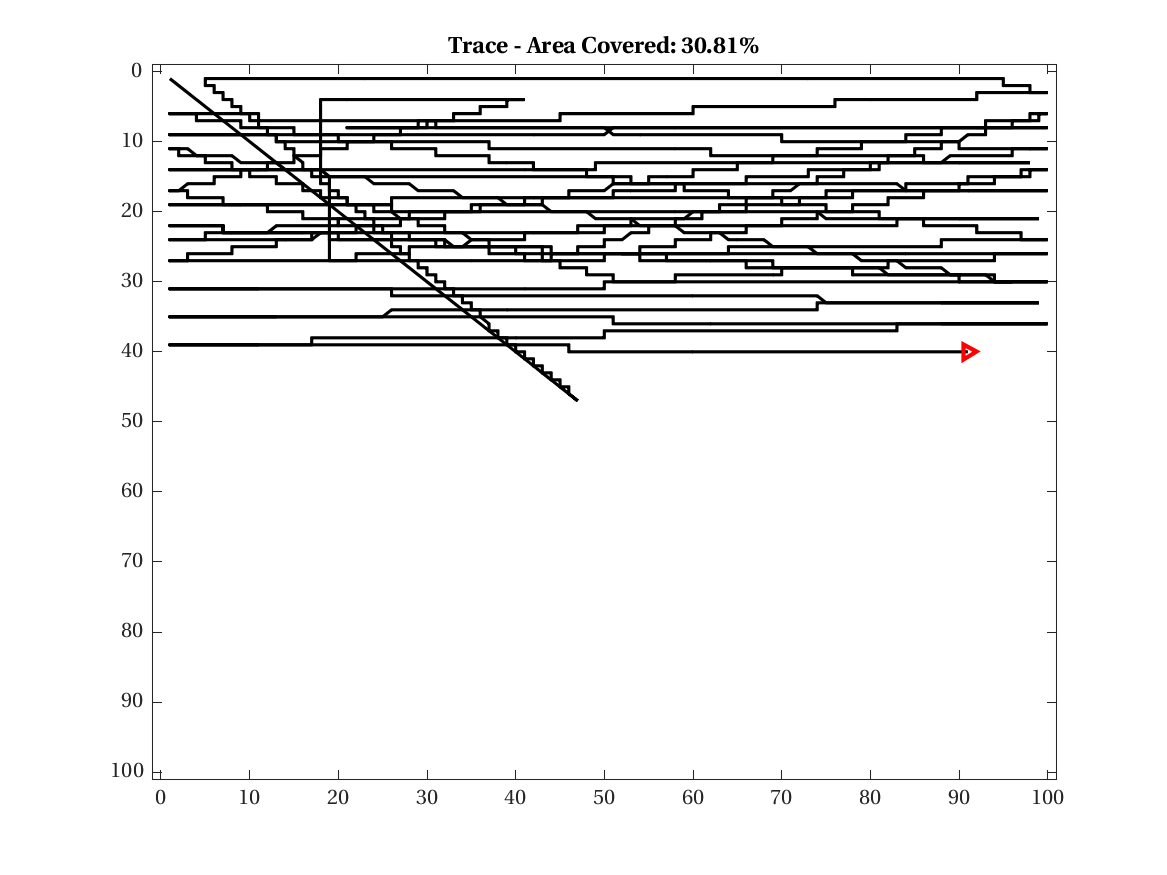
\includegraphics[width=\linewidth]{figures/hbresults/path_nnhv_30p_100x100_sf_1_seed_2.png}
        \captionsetup{skip=0.20\baselineskip,size=footnotesize}
        \caption{$N$ Highest Variance}
    \end{subfigure}%
    \begin{subfigure}[t]{0.3333\textwidth}
        \centering
        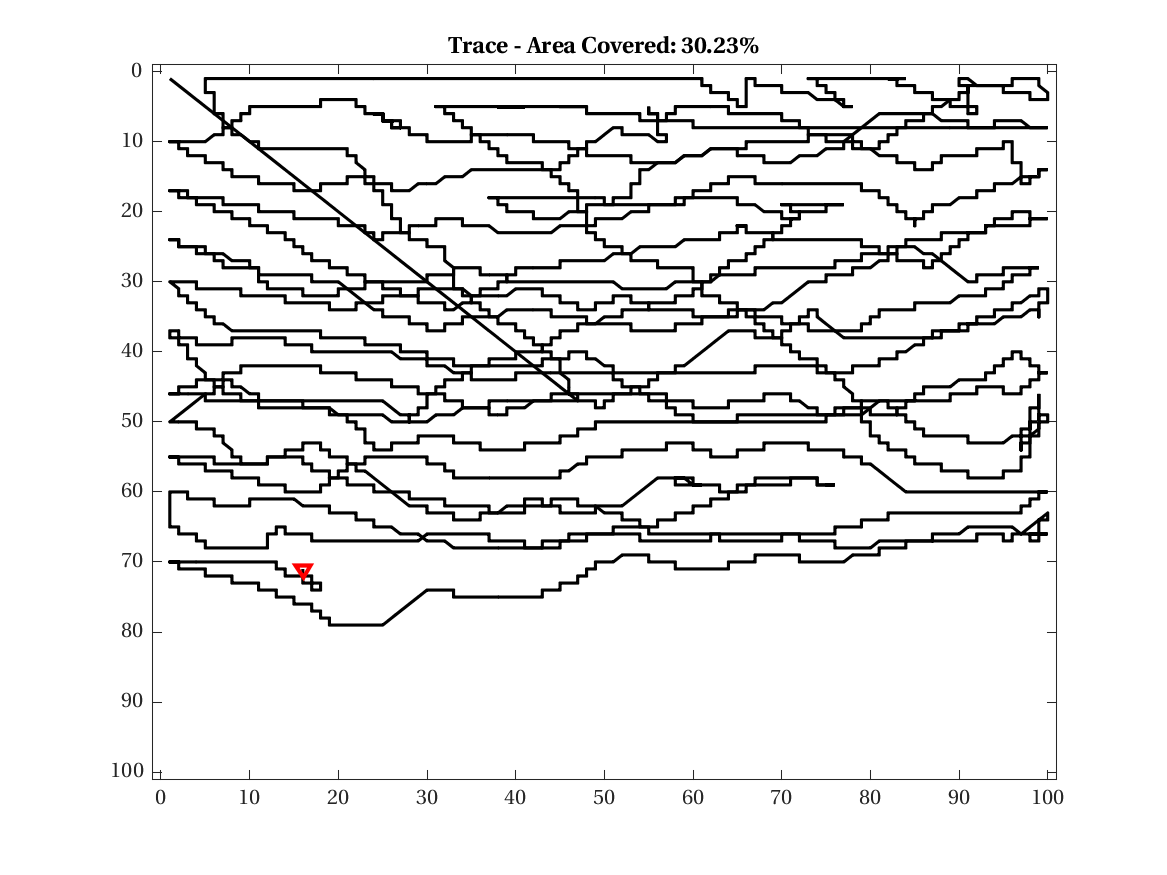
\includegraphics[width=\linewidth]{figures/hbresults/path_mc_30p_100x100_sf_1_seed_2.png}
        \captionsetup{skip=0.20\baselineskip,size=footnotesize}
        \caption{Monte Carlo}
    \end{subfigure}%
    \\
    \begin{subfigure}[t]{0.3333\textwidth}
        \centering
        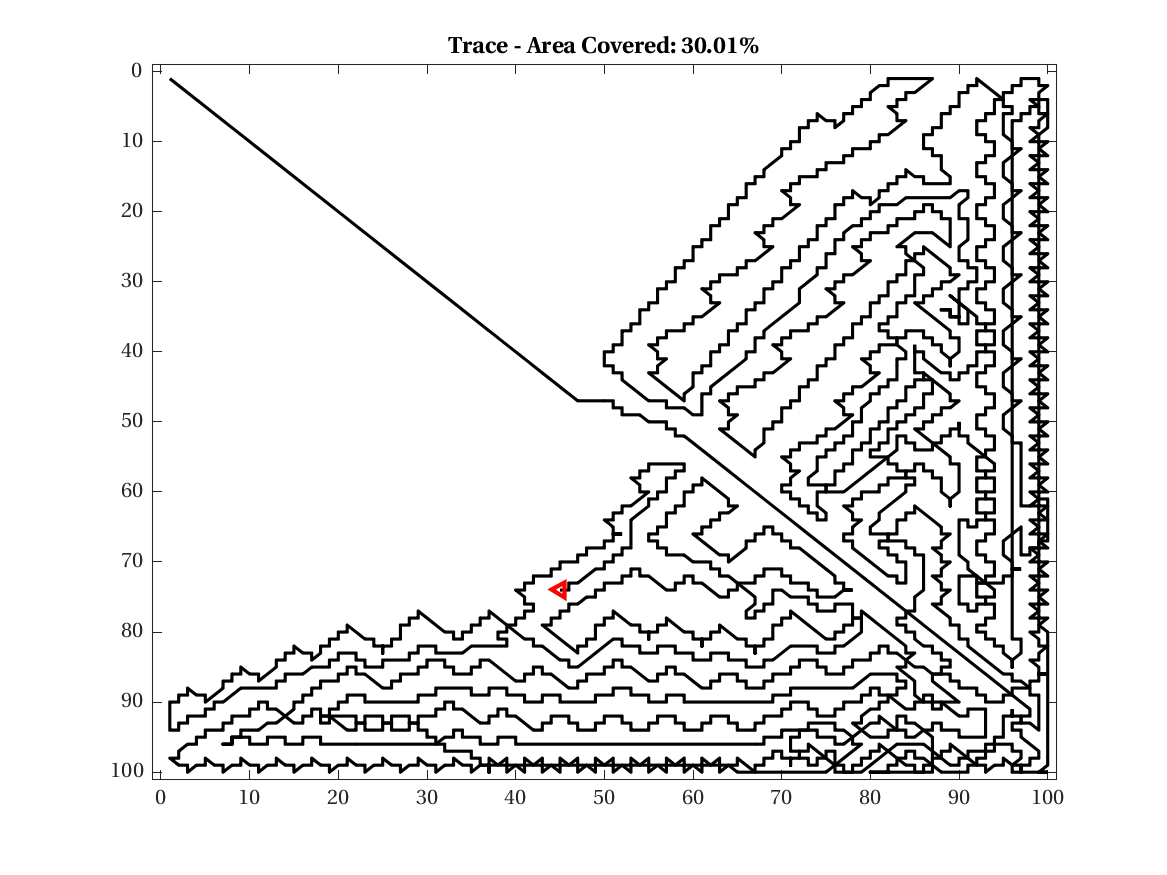
\includegraphics[width=\linewidth]{figures/hbresults/path_gradient_30p_100x100_sf_1_seed_2.png}
        \captionsetup{skip=0.20\baselineskip,size=footnotesize}
        \caption{Gradient Ascent}
    \end{subfigure}%
    \begin{subfigure}[t]{0.3333\textwidth}
        \centering
        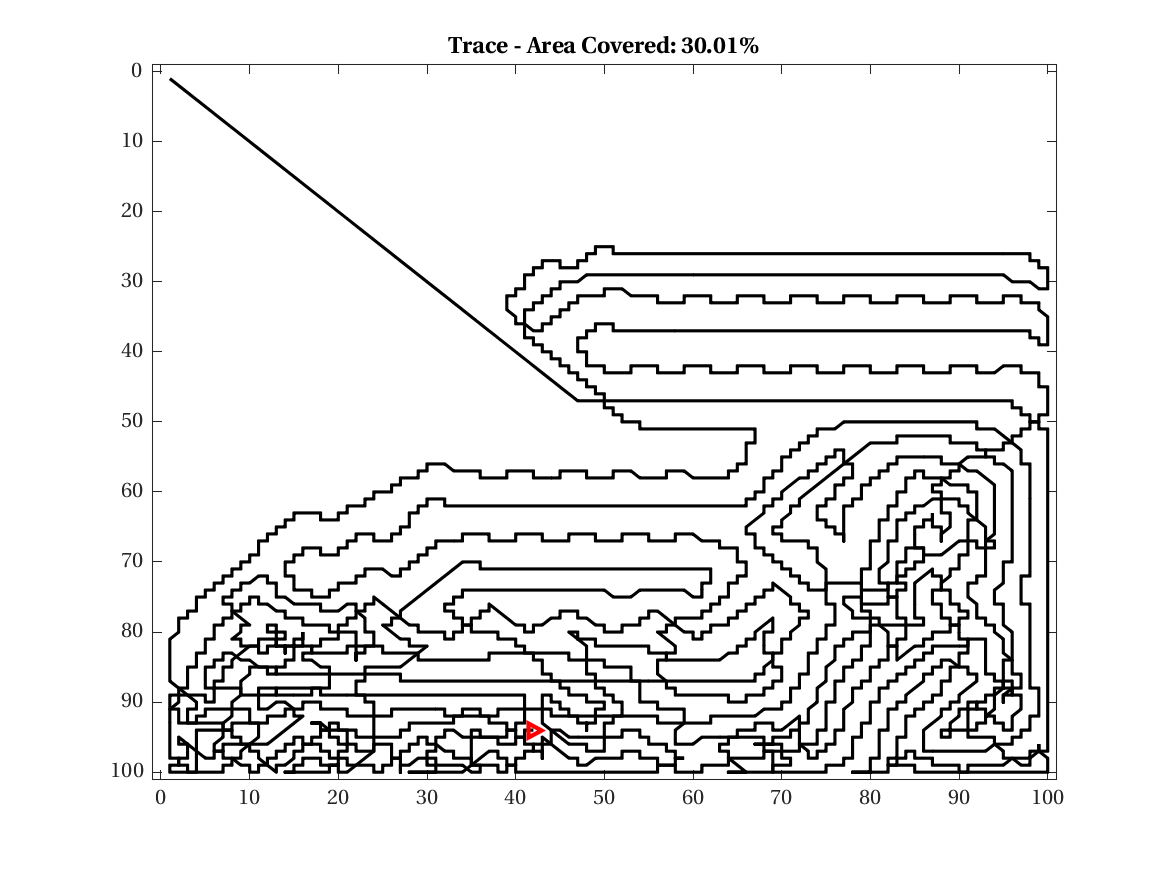
\includegraphics[width=\linewidth]{figures/hbresults/path_gr_30p_100x100_sf_1_seed_2.png}
        \captionsetup{skip=0.20\baselineskip,size=footnotesize}
        \caption{Gradient Range Ascent}
    \end{subfigure}%
    \\
    \begin{subfigure}[t]{0.3333\textwidth}
        \centering
        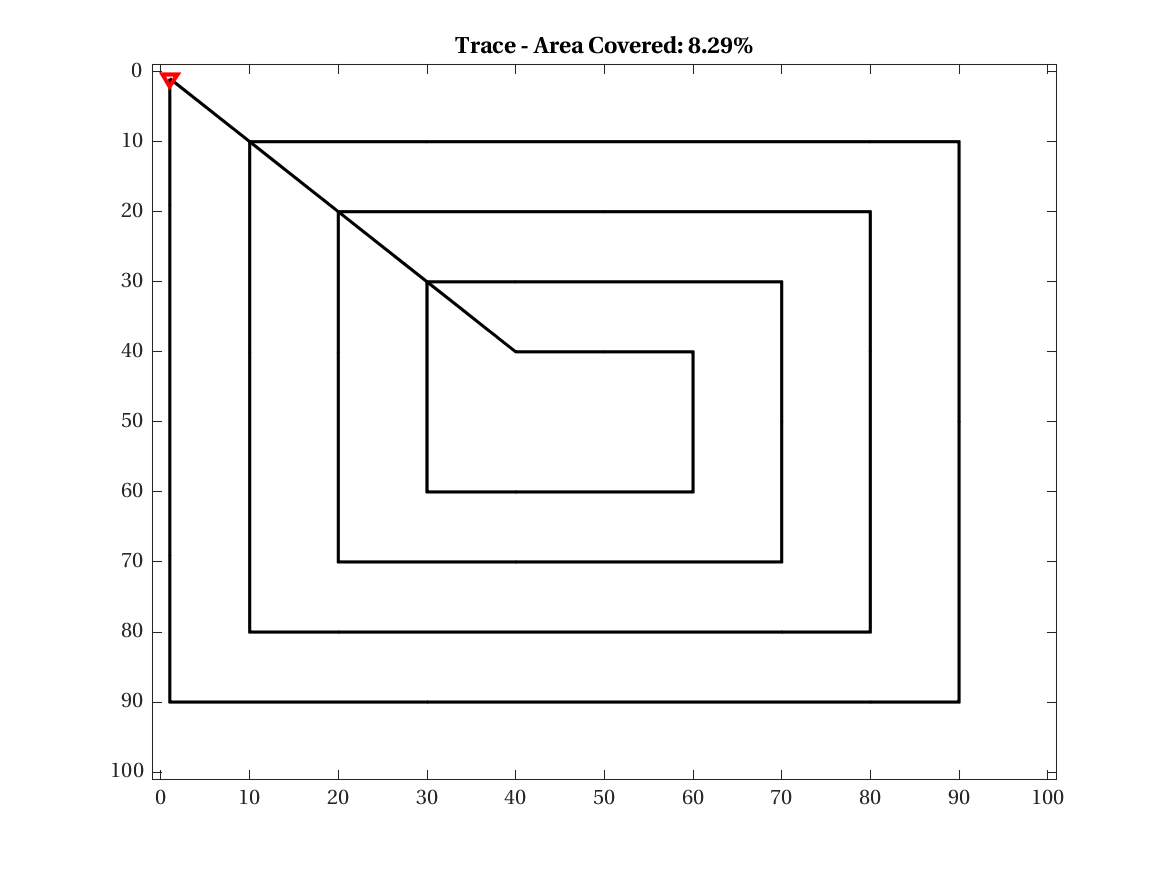
\includegraphics[width=\linewidth]{figures/hbresults/path_zz_10p_100x100_sf_1_seed_2.png}
        \captionsetup{skip=0.20\baselineskip,size=footnotesize}
        \caption{$ZZ_{10}$}
    \end{subfigure}%
    \begin{subfigure}[t]{0.3333\textwidth}
        \centering
        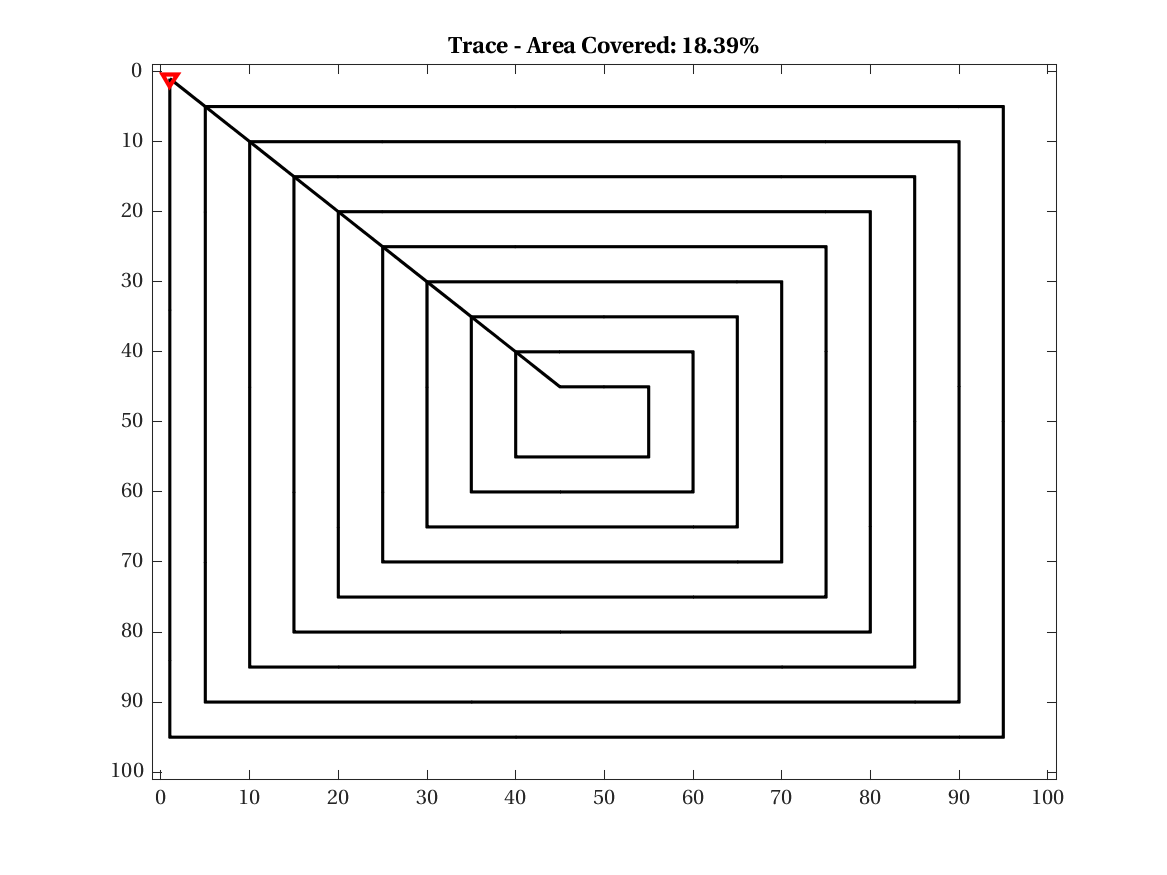
\includegraphics[width=\linewidth]{figures/hbresults/path_zz_20p_100x100_sf_1_seed_2.png}
        \captionsetup{skip=0.20\baselineskip,size=footnotesize}
        \caption{$ZZ_{20}$}
    \end{subfigure}%
    \begin{subfigure}[t]{0.3333\textwidth}
        \centering
        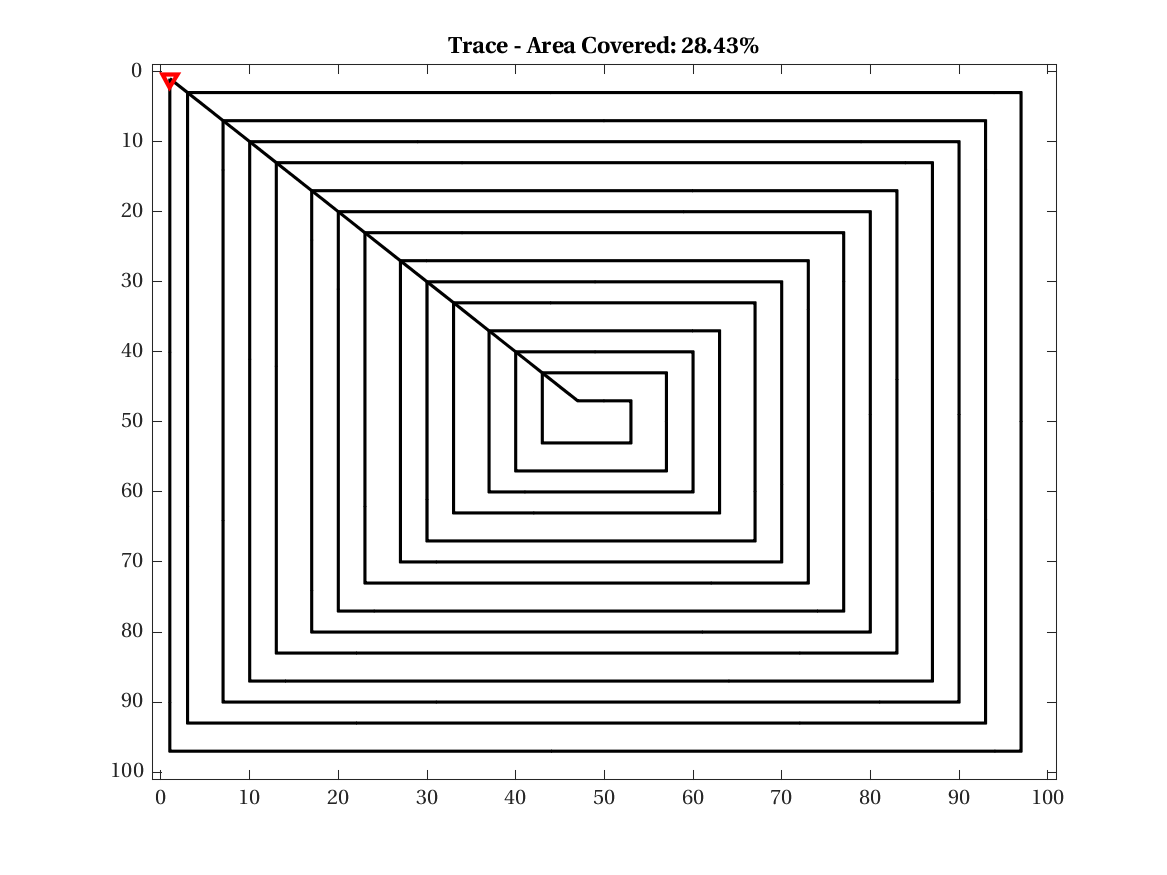
\includegraphics[width=\linewidth]{figures/hbresults/path_zz_30p_100x100_sf_1_seed_2.png}
        \captionsetup{skip=0.20\baselineskip,size=footnotesize}
        \caption{$ZZ_{30}$}
    \end{subfigure}%
    \captionsetup{skip=0.20\baselineskip}
    \caption{Exploration of a field of size $100 \times 100$, $\sigma_{field} = 1$, random seed 2.}
    \label{fig:sf1}
\end{figure}

\begin{figure}[htb!]
    \centering
    \begin{subfigure}[t]{0.75\textwidth}
        \centering
        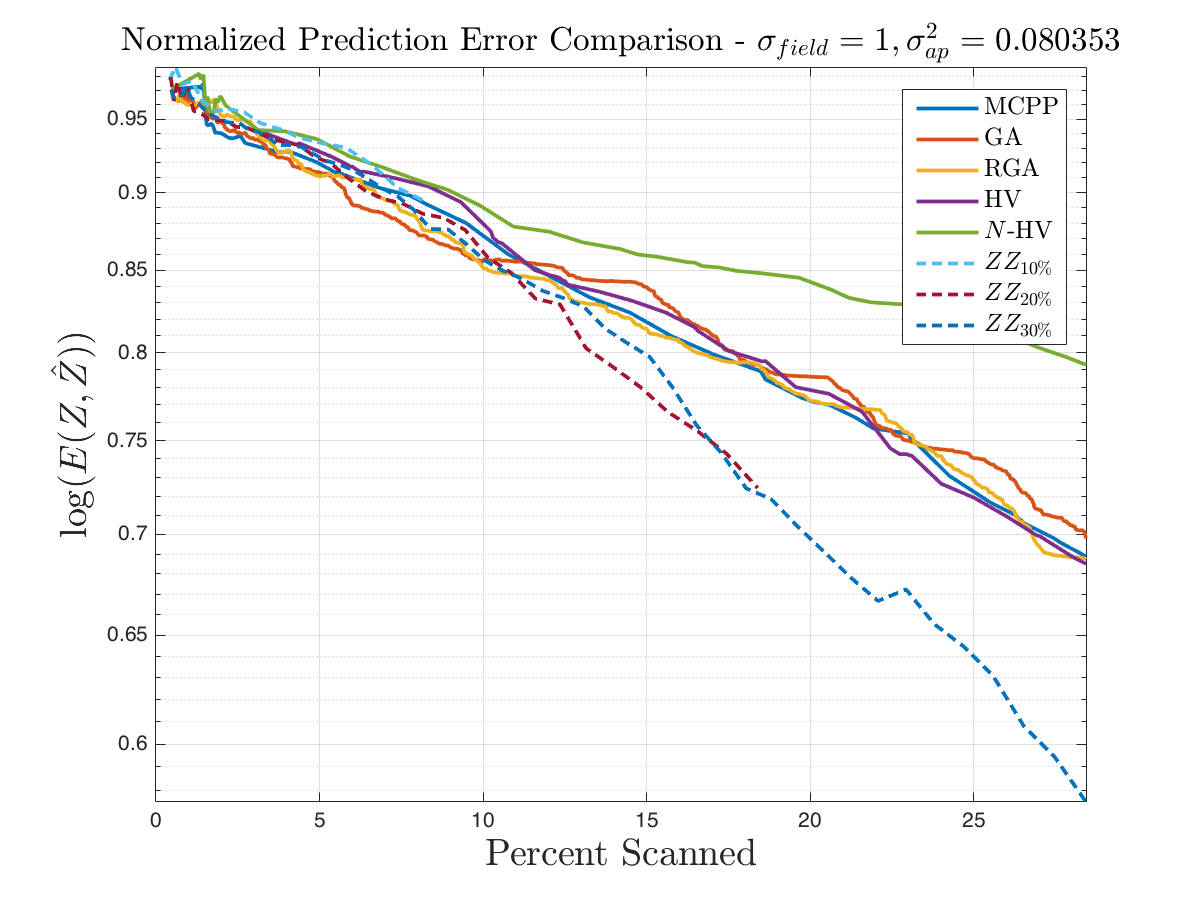
\includegraphics[width=\linewidth]{figures/results/normalized_errors_30p_100x100_sf_1_seed_2_app_50.png}
        \captionsetup{skip=0.20\baselineskip,size=footnotesize}
        \caption{Normalized prediction errors for each method.}
    \end{subfigure}%
    \\
    \begin{subfigure}[t]{0.75\textwidth}
        \centering
        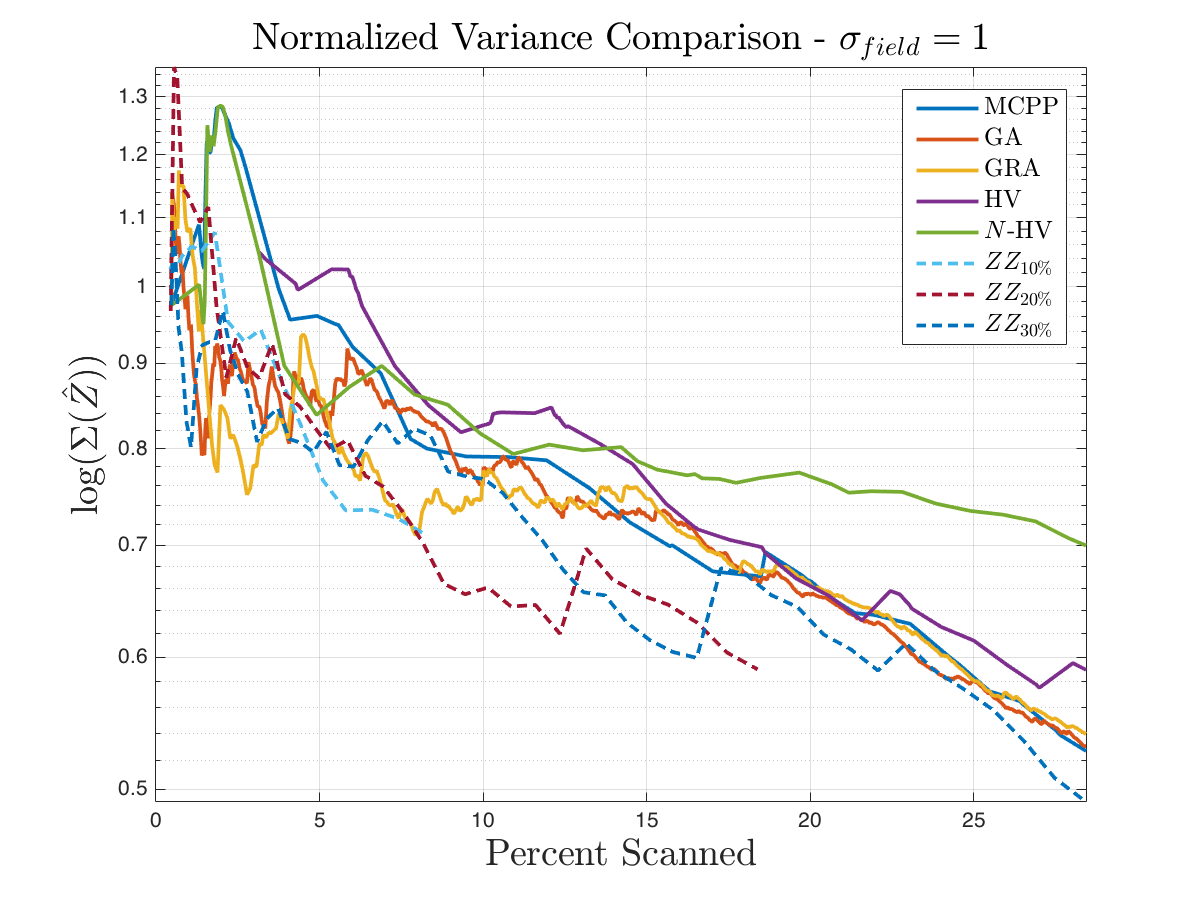
\includegraphics[width=\linewidth]{figures/results/normalized_variances_30p_100x100_sf_1_seed_2_app_50.png}
        \captionsetup{skip=0.20\baselineskip,size=footnotesize}
        \caption{Normalized prediction variances for each method.}
    \end{subfigure}%
    \captionsetup{skip=0.20\baselineskip}
    \caption{Prediction error and variances for an exploration of a field of size $100 \times 100$, $\sigma_{field} = 1$, random seed 2.}
    \label{fig:errvar1}
\end{figure}

\FloatBarrier
\clearpage